\documentclass{beamer}
\usepackage[pangram]{blindtext}
%\usetheme{Pittsburgh}
\usepackage[utf8]{inputenc}
\usepackage[T1]{fontenc}
\usepackage{graphicx}
\usepackage{tikz}
\usetikzlibrary{positioning, fit}
\usetikzlibrary{calc, angles, intersections, quotes, through}
\usepackage{amsmath}
\usepackage{amssymb}
\usepackage{siunitx}
\usepackage{multirow}
\usepackage{makecell}
\usepackage{longtable}
\setbeamertemplate{caption}[numbered]
%\usepackage{subcaption}
\usepackage{tikz}
\usepackage{listings}
\usetikzlibrary{calc}
\usepackage{listings}
\usepackage{subfig}
\usepackage{ifthen}
\tikzset{point/.style={circle, inner sep=0pt, minimum size=3pt, fill=red}}
\usetikzlibrary{shapes}
\newlength{\pvlength}
\def\RTUpresdef{\string~/RTUpresdef}

\title{Studies of colour flow in top quark pair decays at 13 TeV}
\subtitle{Results at the CMS experiment of the CERN LHC\\\vspace{0.5cm}CMS AN-17-309}
\author{Viesturs Veckalns}
\institute{Rīgas Tehniskā universitāte}
\date{Top Event Modelling and Generators - Physics Meeting, ****, 2019}


\usepackage{xparse,calc}
%\logo{\raisebox{-6cm}{\includegraphics[width=1cm]{CMS_logo_May2014-eps-converted-to.pdf}}}

%\makeatletter
\input{\RTUpresdef/presdefinitions.tex}
\newcommand{\DeltaR}{\ensuremath{\Delta R^{}}\xspace}
\newcommand{\leadingjet}{\ensuremath{j_{1}^{W}}\xspace}%
\newcommand{\scndleadingjet}{\ensuremath{j_{2}^{W}}\xspace}%
\newcommand{\leadingb}{\ensuremath{j_{1}^{b}}\xspace}%
\newcommand{\scndleadingb}{\ensuremath{j_{2}^{b}}\xspace}%
\newcommand{\hadronicb}{\ensuremath{j_{\text{h}}^{b}}\xspace}%
\newcommand{\pullangle}{\ensuremath{\theta_{\text{p}}}\xspace}%
\newcommand{\pullvector}{\ensuremath{\vec{P}}\xspace}%
\newcommand{\pvmag}{\ensuremath{\left|\vec{P}\right|}\xspace}%
\newcommand{\pval}{$p$-value}%

\newcommand{\jettitle}[1]{%
\ifthenelse{\equal{#1}{leading_jet}}{\leadingjet}{}%
\ifthenelse{\equal{#1}{scnd_leading_jet}}{\scndleadingjet}{}%
\ifthenelse{\equal{#1}{leading_b}}{\leadingb}{}%
\ifthenelse{\equal{#1}{scnd_leading_b}}{\scndleadingb}{}%
}%

\newcommand{\countertitle}[1]{%
\ifthenelse{\equal{#1}{leading_jet}}{\scndleadingjet}{}%
\ifthenelse{\equal{#1}{scnd_leading_jet}}{\leadingjet}{}%
\ifthenelse{\equal{#1}{leading_b}}{\scndleadingb}{}%
\ifthenelse{\equal{#1}{scnd_leading_b}}{\leadingb}{}%
}%


\newcommand{\observabletitle}[1]{%
\ifthenelse{\equal{#1}{pull_angle}}{pull angle \pullangle}{}%
\ifthenelse{\equal{#1}{pvmag}}{magnitude of the pull vector \pvmag}{}%
}%

\newcommand{\chargetitle}[1]{%
\ifthenelse{\equal{#1}{allconst}}{all jet constituents}{}%
\ifthenelse{\equal{#1}{chconst}}{only charged jet constituents}{}%
}%

\newcommand{\methodtitle}[1]{%
\ifthenelse{\equal{#1}{nominal}}{\ensuremath{t\overline{t}}\xspace}{}%
\ifthenelse{\equal{#1}{cflip}}{\ensuremath{t\overline{t}\ \text{cflip}}\xspace}{}%
}%

\newcommand{\binningtitle}[1]{% 
  \ifthenelse{\equal{#1}{ORIG}}
             {the original binnning}
             {}%    
  \ifthenelse{\equal{#1}{ATLAS3}}{3 regularly sized bins}{}%
  \ifthenelse{\equal{#1}{SIGMA_0p1}}{the optimised binning with a $\sigma$ factor of 0.1}{}%
  \ifthenelse{\equal{#1}{SIGMA_0p6}}{the optimised binning with a $\sigma$ factor of 0.6}{}%
}%           

\newcommand{\flowtitle}[1]{%
\ifthenelse{\equal{#1}{N}}{particle}{}%
\ifthenelse{\equal{#1}{E}}{energy}{}%
\ifthenelse{\equal{#1}{Pt}}{\ensuremath{p_{T}}\xspace}{}%
}%

\newcommand{\recoleveltitle}[1]{%
\ifthenelse{\equal{#1}{gen}}{generator}{}%
\ifthenelse{\equal{#1}{reco}}{reconstruction}{}%
}%

\newcommand{\modeltitle}[1]{%
\ifthenelse{\equal{#1}{nominal}}{SM}{}%
\ifthenelse{\equal{#1}{cflip}}{colour octet $W$}{}%
}%

\def\customwidth{\textwidth}

%% \ExplSyntaxOn
%% \NewExpandableDocumentCommand{\capitalise}{m}{\tl_mixed_case:n{#1}}
%% \ExplSyntaxOff

\usepackage{xspace}
\usepackage{ptdr-definitions}

\begin{document}
{
  \usebackgroundtemplate{\includegraphics[width=\paperwidth]{\RTUpresdef/pamats1.jpg}}%
  \setbeamertemplate{footline}{}
  \logo{}
  \begin{frame}
    \fitimage{%
      \titlepage
      %\blindenumerate[2]
    }{example-image-a}
  \end{frame}
}

\begin{frame}{Collaborators}
  \begin{itemize}
    \item Martijn Mulders (CERN)
    \item Pedro Silva (CERN)
    \item Markus Seidel (CERN)
  \end{itemize}
\end{frame}

\begin{frame}{Colour flow in \ttbar decays}
  \centering
    \includegraphics[width = 0.9\paperwidth]{presfig/ttbar_cf_labels_en.pdf}
\end{frame}

\section{Methodology}
\section{Pull angle}

An explanation about the coordinate system used at CMS is in order. The CMS uses coordinate system centred on the nominal collision point, the $x$ points towards the centre of the LHC, the $y$ axis points upwards and the $z$ axis points along the beam in the direction of the Jura mountains - see Fig.~\ref{fig:CMScoordinates}. $\rho$ is the radial coordinate. The azimuthal angle $\phi$ is measured from the $x$ axis to the projection of the spatial vector $\textbf{p}$ in the $x-y$ plane. The polar angle $\theta$ is measure from the positive direction of the beam to the vector $\textbf{p}$. Pseudorapidity $\eta$ is defined as

\begin{equation}
\eta\equiv-\ln\left(\frac{\theta}{2}\right).
\end{equation}

The pseudorapidity is equal to

\begin{equation}
\eta=\ln\left(\frac{p+p_{L}}{p-p_{L}}\right),
\end{equation}

where $p$ is the magnitude of $\textbf{p}$ and $p_{L}$ is the longitudinal component of $\textbf{p}$ along the direction of the beam. A measurement related to pseudorapidity is the rapidity $y$ defined as:

\begin{equation}
y\equiv\ln\left(\frac{E+p_{L}}{E-p_{L}}\right),
\end{equation}

where $E$ is the energy of the particle. For massless particles rapidity and pseudorapidity are equal. For our present purposes, rapidity and pseudorapidity can be used interchangeably without a loss of accuracy.

\begin{figure}[hptb]
  \centering
  \includegraphics[width=0.7\textwidth]{fig/coordinates/coordinates.pdf}
  \caption{The coordinate system of CMS.}
  \label{fig:CMScoordinates}
\end{figure}

We adopt the methodology proposed by~\cite{Gallicchio:2010sw} to use the pull angle to reveal colour connection between two quark jets. The pull angle $\theta_{p}$ formed by the pull vector $\vec{v}_{p}$ and difference between two jets $\vec{J}_{2}-\vec{J}_{1}$ is shown in Fig.~\ref{fig:pull_angle}. The $\phi$-$y$ coordinate system is used. 

\begin{figure}[hbtp]
  \centering
  \includegraphics[width=1.0\textwidth]{fig/pull_angle.pdf}
  \caption{Pull angle $\theta_{p}$, pull vector $\vec{v}_{p}$ in a $y$-$\phi$ plane.}
  \label{fig:pull_angle}
\end{figure}

The pull vector is given by the formula

\begin{equation}
  \vec{v}_{p}=\sum_{i\in J}\frac{p^{i}_{T}|\vec{r}_{i}|}{p^{J}_{T}}\vec{r}_{i},
  \label{Eq:pull_angle}
\end{equation}

where $i$ is the index of the constituent of jet $J$, $p^{i}_{T}$ is the transverse moment of the jet constituent, $\vec{r}_{i}$ is the vectorial difference between the jet component and the jet, $p^{J}_{T}$ - the transverse moment of the jet.

Two jets that are colour connected are expected to have jet constituents dispersed in the area between the two jets. Hence the pull vector of $J_{1}$ would point towards $J_{2}$ and the pull angle would be narrow. For jets that are not colour connected the pull angle is expected to be distributed isotropically.

The methodology of the pull angle has been applied in the \DZERO experiment of Tevatron~\cite{Abazov:2011vh} and the ATLAS experiment at the LHC in Run I~\cite{Aad:2015lxa} and in Run II~\cite{ATLAS:2017iaz}. We hope to outperform all results with the methodology of the pull angle with the state-of-the-art tracker of the CMS detector immersed in the 4~T magnetic field of the superconducting solenoid.

The anti-$k_{T}$ clustering algorithm ensures a conical jet shape in case the jet separation \DeltaR is more than double of the parameter $R$, which is set at 0.4 at CMS. This case is illustrated in Fig.~\ref{fig:anti_kt_a}. In case of separation between jets \DeltaR being less than double of the parameter $R$ the hard jet will wean constituents from the soft jet. This is illustrated in Fig.~\ref{fig:anti_kt_b}. This latter effect will have consequences for the colour flow analysis with the pull angle as it will induce a pull from the involved jets to each other. This warrants a separation of the cases $\DeltaR\leq2R$, $\DeltaR>2R$. 

\begin{figure}[hbtp]
  \def\twidth{0.5}
  \subfloat[$\Delta_{ij}=3.15$.]{
    \includegraphics[width=\twidth\textwidth]{fig/dR-3p150-pt2-075.pdf}
    \label{fig:anti_kt_a}
  }%
 \subfloat[$\Delta_{ij}=1.95$.]{
    \includegraphics[width=\twidth\textwidth]{fig/dR-1p950-pt2-075.pdf}
    \label{fig:anti_kt_b}
  }
   \caption{Jet shapes obtained with the anti-$k_{T}$ clustering. $R=1.5$ is used. Two cases are shown - $\Delta_{ij}=3.15$ and  $\Delta_{ij}=1.95$. The \pt of the hard jet is 100~\GeV, the \pt of the soft jet is 75~\GeV. Courtesy of Cacciari, Salam and Soyez~\cite{github:antikt}.}
  \label{fig:anti_kt}
\end{figure}

Tracking efficiency of the detector is not perfect. It depends on the quality of the track finder algorithm and properties of the detector such as geometrical acceptance and material content. Fig.~\ref{fig:2011_trackPerformance_MC_SingleParticles_pi_efficiencyVsPt} shows the tracking efficiency of pions, a particle commonly resulting from quark hadronisation. Tracking efficiency is defined as the fraction of simulated charged particles that can be associated with corresponding reconstructed tracks. The tracking efficiency drops at low \pt of the particle. In our analysis we choose 1.0~\GeV as the threshold and exclude particles whose \pt is below it from our analysis.

\begin{figure}[hbtp]
    \includegraphics[width=0.6\textwidth]{fig/figs_2011_trackPerformance_MC_SingleParticles_pi_efficiencyVsPt.png}
    \caption{Track reconstruction efficiencies for pions passing the high-purity quality requirements. Results are shown as a function of \pt, for the barrel, transition, and endcap regions, which are defined by the $\eta$ intervals of 0-0.9, 0.9-1.4 and 1.4-2.5, respectively~\cite{Chatrchyan:2014fea}.}
    \label{fig:2011_trackPerformance_MC_SingleParticles_pi_efficiencyVsPt}
\end{figure}

\section{LEP method}

Another methodology of studying colour-connected jets in the process $e^{+}e^{-}\rightarrow q\overline{q}q\overline{q}$ at \sqrts=189-207~\GeV was used in various experiments of LEP~(\cite{Abdallah:2006uq}, \cite{Abbiendi:2005es}, \cite{Achard:2003pe}). Two inter-\PW planes formed by colour-connected quarks and two intra-\PW planes formed by quarks that are not colour connected are introduced as shown in Fig.~\ref{fig:LEP_method}. Particles are projected onto these planes and the angle with the leftmost quark $\chi_{1}$ is taken. If this angle is less than the angle $\chi_{0}$ between the quarks forming the plane (which means the particle is projected between the respective quarks) then the normalised angle $\chi_{R}=\frac{\chi_{1}}{\chi_{0}}$ is plotted in the region corresponding to the plane after a linear transformation

\begin{equation}
  \chi=\chi_{R}+n_{\text{plane}}-1
\end{equation}

has been performed on the normalised angle. 

\begin{figure}[hbtp]
  \centering
  \includegraphics[width=0.6\textwidth]{fig/L3method.pdf}
  \caption{Inter-\PW and intra-\PW planes in the process $e^{+}e{-}\rightarrow q\overline{q}q\overline{q}$ and the relative angle $\chi_{R}=\frac{\chi_{1}}{\chi_{0}}$.}
  \label{fig:LEP_method}
\end{figure}

In the \ttbar semileptonic decay an arrangament as shown in Fig.~\ref{fig:LEP_method} is not possible. Therefore a modification as shown in Fig.~\ref{fig:LEP_method_adaptation} is proposed. There is one plane formed by colour connected jets - the leading light jet \leadingjet and the second leading light jet \scndleadingjet from the hadronic decay of the \PW boson. Additionally there are 3 colour-free regions formed by 1) the furthest light jet $j^{\PW}_{f}$ and the hadronic \cPqb jet \hadronicb 2) the hadronic \cPqb jet \hadronicb and the closest light jet $j^{\PW}_{c}$, 3) the leading \cPqb jet \leadingb and the second leading \cPqb jet \scndleadingb. Whether a jet is close or far is determined with regard to the angle between jets in the Euclidian space. In the regions shown in Fig.~\ref{fig:LEP_method_adaptation_qfhb} and Fig.~\ref{fig:LEP_method_adaptation_hbqc} we may hope to observe colour reconnection effects.

\begin{figure}[hbtp]
  \centering
  \def\twidth{0.24}
  \subfloat[Colour-connected region \leadingjet-\scndleadingjet.]{%
    \includegraphics[width=\twidth\textwidth]{fig/LEP_adaptation/qlq2l.pdf}%
    \label{fig:LEP_method_adaptation_qlq2l}
  }\hfil
 \subfloat[Colour-free region $j^{\PW}_{f}$-\hadronicb.]{%
    \includegraphics[width=\twidth\textwidth]{fig/LEP_adaptation/qfhb.pdf}%
    \label{fig:LEP_method_adaptation_qfhb}
 }\hfil
  \subfloat[Colour-free region \hadronicb-$j^{W}_{c}$.]{%
    \includegraphics[width=\twidth\textwidth]{fig/LEP_adaptation/hbqc.pdf}%
    \label{fig:LEP_method_adaptation_hbqc}
  }\hfil
  \subfloat[Colour-free region \leadingb-\scndleadingb.]{%
    \includegraphics[width=\twidth\textwidth]{fig/LEP_adaptation/blb2l.pdf}%
    \label{fig:LEP_method_adaptation_blb2l}
  }
  \caption{Adaptation of the LEP method to \ttbar semileptonic decay involving a colour-connected region and 3 colour-free regions.}
  \label{fig:LEP_method_adaptation}
\end{figure}

The method calls for a separation of hadronic and leptonic \cPqb quarks. Each \cPqb quark is paired to each \PW boson and the invariant mass is compared to the mass of the \cPqt quark - 173.34~\GeV. The \cPqb quark is assigned to the branch where the difference of the masses is the smallest. 


\begin{frame}{Colour octet \PW boson}
  \centering
  \includegraphics[width=0.7\textwidth]{fig/ttbar_cf_flip_cropped.pdf}
\end{frame}

\section{Event Selection}
Notikumu atlases mērķis ir nodalīt signālu no fona. Notikumu atlase ir atšķirīga detektora līmeņa MK notikumiem un ģeneratora līmeņa MK notikumiem. Dati tiek atlasīti atbilstoši detektora līmeņa notikumu atlasei.

Šīs nodaļas izklāsts ir pielāgots pēc~\cite{CMS-AN-2017-159} parauga, jo šajā pētījumā tiek izmantota līdzīga notikumu atlase.

\section{Detektora līmenis}
\label{sec:detector_level}

Notikumu atlase ir balstīta \ttbar$\to$ leptons + strūklas topoloģijā, kur viens no \PW bozoniem sabrūk par lādētu leptonu ($\ell=e, \mu$) un atbilstošo neitrino, bet otrs \PW bozons sabrūk par kvarkiem, kas rada strūklas.

Lai rekonstruētu gala stadijas objektus, tiek izmantots daļiņu plūsmas algoritms~\cite{Sirunyan:2017ulk}. Lai celtu rekonstrukcijas kvalitāti, šis algoritms kombinē signālus no visiem apakšdetektoriem, un ar tā palīdzību var identificēt mionus, elektronus, fotonus, lādētos hadronus un neitrālos hadronus pēc \Pp\Pp sadursmes.

Datu paraugi tiek ievākti, izmantojot \gls{Augsta līmeņa trigera} viena leptona trigera ceļus, kas apkopoti \ref{tab:triggers}~tab.

\begin{table}[htp]
\centering
\caption{Analīzē izmantotās tiešsaistes atlases trigera ceļi.}
\label{tab:triggers}
\begin{tabularx}{\linewidth}{lllXX}\hline
Gala stadija                & Ceļš                                       & Darbības intervāls & Funkcija & L1 sākums\\\hline
$e$ + strūklas                      & \small HLT\_Ele32\_eta2p1\_WPTight\_Gsf\_v & visi       & \small Atlasīt $e$ ar $\left|\eta\right|<2,1$ un $\pt>32~\GeV$ ciešajā darbības punktā, izmantojot GSF, lai rekonstruētu trekus
                                                                                         & \small L1\_SingleEG40\newline VAI\newline L1\_SingleIsoEG22er\newline VAI\newline L1\_SingleIsoEG24er\newline VAI\newline L1\_SingleIsoEG24\newline VAI\newline L1\_SingleIsoEG26\\\hline
\multirow[t]{2}{*}{$\mu$ + strūklas}
                            & \small HLT\_IsoMu24\_v                     & visi       & \small Atlasīt izolētu $\mu$ ar $\pt>20$~\GeV, izmantojot L3 trekera algoritmu
                                                                                         & \multirow[t]{2}{*}{\small L1\_SingleMu18}\\
                            & \small HLT\_IsoTkMu24\_v                   & visi       & \small Atlasīt izolētu $\mu$ ar $\pt>20$~\GeV, izmantojot HLT trekera mionu algoritmu
                            & \\\hline
\end{tabularx}
\end{table}

Bezsaistē tiek prasīts viens ciešs elektrons/mions ar $\pt>34/26~\GeV$ un $|\eta|<2,1/2,4$. Notikumam, kurā ir otrs vaļīgs leptons ar $\pt>15~\GeV$ un $|\eta|<2,4$, tiek uzlikts veto.

Notikumā jābūt četrām strūklām, kas sakopotas ar anti-$k_{\text{T}}$ algoritmu, strūklu atdalījumu ar $R=0,4$ un lādēto hadronu atņemšanu (AK4PFchs) un kurām $\pt>30\GeV$ un $|\eta|<2,4$. 

Vismaz divām strūklām jābūt \cPqb atzīmētām ar {\it Combined Secondary Vertex} algoritma (CSVv2) vidējo darbības punktu. 

Notikumā jābūt vismas divām neatzīmētām (vieglajām) strūklām, kurām jārada \PW bozona kandidāts, kura invariantā masa $\left|m_{jj}-80,4\right|<15~\GeV$.

Notikumu raža dažādās atlases stadijās ir redzama \ref{fig:_reco_selection}~att. un sniegta \ref{tab:yields}~tab. \ref{tab:yields_cflip}~tab. attēlota notikumu raža krāsu okteta \PW paraugam. Signāla īpatsvars palielinās no 0,1~\% sākotnējā stadijā līdz 94,2~\% gala stadijā \textendash\ tas ir šīs atlases efektivitātes mērs.

\figureEML{/reco/}{_reco_selection}{Notikumu raža dažādās notikumu atlases stadijās: $1 \ell$, $1 \ell + \geq 4 j$, $1 \ell + \geq 4 j (2 b)$, $1 \ell + \geq 4 j (2 b, 2 lj)$.}

\input{tables/event_yields_tableslv/event_yields_table.txt}

\input{tables/event_yields_tableslv/event_yields_table_cflip.txt}

\section{Ģeneratora līmenis}
\label{sec:generator_level}

Simulācijā bezsaistes atlase daļiņu līmenī tiek imitēta, izmantojot \PSEUDOTOPPRODUCER rīku~\cite{code:pseudotop}, izmantojot kopīgu leptonu atlasi gan elektroniem, gan mioniem ar $\pt>26\GeV$ un $|\eta|<2,4$, kā arī tādām pašām prasībām strūklām $\pt/\eta$ ($\pt>30~\GeV$, $|\eta|<2,4$) un \PW masai ($\left|m_{jj}-80,4\right|<15~\GeV$) kā bezsaistes atlasei detektora līmenī.

Lādētie leptoni, kas izdalās cietajā procesā, tiek apzaroti ar leptoniem $R=0,1$ konusā. Strūklas tiek sakopotas ar anti-$k_\text{T}$ algoritmu ar $R=0,4$ konusu pēc apzaroto leptonu kā arī visu neitrino noņemšanas. Lai noteiktu strūklas smaržu daļiņu līmenī, strūklas sakopojumā tiek iekļauti ``spoku'' $B$ hadroni, kad to moments ir reizināts ar $10^{-20}$ tā, lai tie būtiski nemainītu strūklas enerģijas mērogu daļiņu līmenī.


\section{Corrections and systematics}
\input{presxxx/systematics.tex}

\section{Results}
\label{chap:results}
\section{Event display}
A selected event is displayed in Fig. \ref{fig:event_display}, showing the light jets and the pull vector in the $\eta - \phi$ plane in a manner analogous to Fig. \ref{fig:pull_angle}.

\begin{figure}[hbtp]
  \centering
  \includegraphics[width=1.0\textwidth]{fig/individual_plots/reco_allconst_total_1111_DeltaR_2p846131_pull_angle_1p964620.png}
  \caption{Pull vector (dash-dotted) of the leading jet forming a pull angle of 1.96 rad with the difference between the second leading jet and the leading jet (dashed). Constituents of the leading jet are marked in blue while the constituents of the second leading jet ar marked in red. The leading jet is marked with a solid line while the second leading jet is marked with a dotted line. The pull vector is enhanced 200 times, while the radius of the circles representing jets is equal to $\frac{p_{T}}{75.0}$ and the radius of the circles representing constituents is equal to $\frac{p^{\text{constituent}}_{T}}{p^{\text{jet}}_{T}}$.}
  \label{fig:event_display}
\end{figure}

\section{Pull vector}

A set of base tools \textsc{CFAT} \cite{url:cfat} was developed having in mind that the analysis can be implemented both in \RIVET and \CMSSW. Initial tests were done with \RIVET because before the colour octet \PW samples were developed this procedure provided the only means to generate colour-flipped events. Results with \RIVET are shown in Fig. \ref{fig:resultsRivet}. Fig. \ref{fig:pull_angle_allconst_Rivet_leading_jet_2nd_leading_jet_DeltaRTotal_4j2t} shows the distribution of \pullangle between \leadingjet and \scndleadingjet. The central peak which is the experimental signature of colour connect jets is present in the SM results but disappears in the \PW colour octet results. On the other hand the distribution of \pullangle suffers no alterations between \leadingjet and lepton as shown in Fig. \ref{fig:pull_angle_allconst_Rivet_leading_jet_lepton_DeltaRTotal_4j2t}.

\begin{figure}[htp]
\centering
  \def\twidth{0.45}
  \centering
  \subfloat[Distribution of \pullangle from \leadingjet to \scndleadingjet.]{
    \includegraphics[width=\twidth\textwidth]{fig/pull_angle_allconst_Rivet_leading_jet_2nd_leading_jet_DeltaRTotal_4j2t.png}
    \label{fig:pull_angle_allconst_Rivet_leading_jet_2nd_leading_jet_DeltaRTotal_4j2t}
  }%
  \subfloat[Distribution of \pullangle from \leadingjet to lepton.]{
    \includegraphics[width=\twidth\textwidth]{fig/pull_angle_allconst_Rivet_leading_jet_lepton_DeltaRTotal_4j2t.png}
    \label{fig:pull_angle_allconst_Rivet_leading_jet_lepton_DeltaRTotal_4j2t}
  }
\caption{Results with \RIVET showing SM (blue) and \PW colour octet (red) distributions of the pull angle. The bottom inset shows the bin-per-bin ratio of the \PW colour octet results to the SM results.}
\label{fig:resultsRivet}
\end{figure}

A more comprehensive analysis with data and simulated events at generator and reconstruction level was implemented in \CMSSW version \lstinline[language=sh]|CMSSW_8_0_26_patch1|. The plots are rendered with \ROOT \cite{Brun}. The pull vectors were obtained for all observable jets - the leading light jet \leadingjet (highest \pt), the second leading light jet \scndleadingjet, the leading hadronic $b$ jet \leadingb and the second leading hadronic $b$ jet \scndleadingb. In each case it was diffentiated whether all jet particles or only charged ones should be included in determining the pull jet. The results are separated into $e$ + jets, $\mu$ + jets and combined lepton + jets channels.

The $\eta$ dimension of the pull vector with all jet components is given in Fig. \ref{fig:_eta_PV_allconst_reco_leading_jet} - \ref{fig:_eta_PV_allconst_reco_leading_jet}.

An explanation of how CMS plots are represented is in order. The top plot in Fig. \ref{fig:_eta_PV_allconst_reco_leading_jet} shows data and Monte Carlo simulations. Unless otherwise specified the Monte Carlo is in reconstruction level. The blue band shows systematics. Given a systematic with index $k$ we identify it as an upside systematic $U^{k}_{i}$ if in bin $i$ the systematic $S^{k}_i$ exceeds the nominal value $N_{i}$. In the opposide case we classify the systematic as a downside systematic $D^{k}_{i}$. The total upside and downside systematic is given as a sum of squares:

\begin{align}
U_{i}=\sqrt{\sum_{k}\left(U^{k}_{i}-N_{i}\right)^{2}} && D_{i}=\sqrt{\left(\sum_{k}D^{k}_{i}-N_{i}\right)^{2}}.
\end{align}

The width of the blue band corresponds to the systematical error calculated as $\frac{U_{i}+D_{i}}{2}$. It is centred on $N_{i} + \frac{U_{i}-D_{i}}{2}$. The same applies to the pink band except that the systematics are normalised to the integral of the signal (such normalised histograms are referred to as shapes). The bottom inset shows the ratio of data to Monte Carlo, as well as systematics and systematics fom shapes normalised to Monte Carlo.

\figureEML{/reco/PV/charge/allconst/}
          {_eta_PV_allconst_reco_leading_jet}
          {$\eta$ dimension of the pull vector of \leadingjet with all jet components.}
\figureEML{/reco/PV/charge/allconst/}
          {_eta_PV_allconst_reco_scnd_leading_jet}
          {$\eta$ dimension of the pull vector of \scndleadingjet with all jet components.}
\figureEML{/reco/PV/charge/allconst/}
          {_eta_PV_allconst_reco_leading_b}
          {$\eta$ dimension of the pull vector of \leadingb with all jet components.}
\figureEML{/reco/PV/charge/allconst/}
          {_eta_PV_allconst_reco_scnd_leading_b}
          {$\eta$ dimension of the pull vector of \scndleadingb with all jet components.}

The $\phi$ dimension of the pull vector with all jet components is given in Fig. \ref{fig:_phi_PV_allconst_reco_leading_jet} - \ref{fig:_phi_PV_allconst_reco_leading_jet}. 

\figureEML{/reco/PV/charge/allconst/}
          {_phi_PV_allconst_reco_leading_jet}
          {$\phi$ dimension of the pull vector of \leadingjet with all jet components.}
\figureEML{/reco/PV/charge/allconst/}
          {_phi_PV_allconst_reco_scnd_leading_jet}
          {$\phi$ dimension of the pull vector of \scndleadingjet with all jet components.}
\figureEML{/reco/PV/charge/allconst/}
          {_phi_PV_allconst_reco_leading_b}
          {$\phi$ dimension of the pull vector of \leadingb with all jet components.}
\figureEML{/reco/PV/charge/allconst/}
          {_phi_PV_allconst_reco_scnd_leading_b}
          {$\phi$ dimension of the pull vector of \scndleadingb with all jet components.}

The magnitude of the pull vector with all jet components is given in Fig. \ref{fig:_mag_PV_allconst_reco_leading_jet} - \ref{fig:_mag_PV_allconst_reco_leading_jet}. The magnitude of the pull vector is usually contained below 0.02 [a.u.].

\figureEML{/reco/PV/charge/allconst/}
          {_mag_PV_allconst_reco_leading_jet}
          {The magnitude dimension of the pull vector of \leadingjet with all jet components.}
\figureEML{/reco/PV/charge/allconst/}
          {_mag_PV_allconst_reco_scnd_leading_jet}
          {The magnitude dimension of the pull vector of \scndleadingjet with all jet components.}
\figureEML{/reco/PV/charge/allconst/}
          {_mag_PV_allconst_reco_leading_b}
          {The magnitude dimension of the pull vector of \leadingb with all jet components.}
\figureEML{/reco/PV/charge/allconst/}
          {_mag_PV_allconst_reco_scnd_leading_b}
          {The magnitude dimension of the pull vector of \scndleadingb with all jet components.}

\section{Pull angle}

The plots of the pull angle between colour connected jets - \leadingjet to \scndleadingjet and \scndleadingjet to \leadingjet with all jet constituents and including all values of $\Delta R$ are shown in Fig. \ref{fig:_pull_angle_allconst_reco_leading_jet_scnd_leading_jet_DeltaRTotal} and Fig. \ref{fig:_pull_angle_allconst_reco_scnd_leading_jet_leading_jet_DeltaRTotal}.

\figureEML{/reco/pull_angle/DeltaRTotal/charge/allconst/}
          {_pull_angle_allconst_reco_leading_jet_scnd_leading_jet_DeltaRTotal}
          {Pull angle distribution of \leadingjet to \scndleadingjet for all \DeltaR and including all particles.}

\figureEML{/reco/pull_angle/DeltaRTotal/charge/allconst/}
          {_pull_angle_allconst_reco_scnd_leading_jet_leading_jet_DeltaRTotal}
          {Pull angle distribution of \scndleadingjet to \leadingjet for all \DeltaR and including all particles.}

Additionally, the plots of the pull angle between jets where we expect no colour connection - \leadingb to \scndleadingb and \scndleadingb to \leadingb with all jet constituents and including all values of $\DeltaR $ are shown in Fig. \ref{fig:_pull_angle_allconst_reco_leading_b_scnd_leading_b_DeltaRTotal} and Fig. \ref{fig:_pull_angle_allconst_reco_scnd_leading_b_leading_b_DeltaRTotal}.

\figureEML{/reco/pull_angle/DeltaRTotal/charge/allconst/}
          {_pull_angle_allconst_reco_leading_b_scnd_leading_b_DeltaRTotal}
          {Pull angle distribution of \leadingb to \scndleadingb for all \DeltaR and including all particles.}

\figureEML{/reco/pull_angle/DeltaRTotal/charge/allconst/}
          {_pull_angle_allconst_reco_scnd_leading_b_leading_b_DeltaRTotal}
          {Pull angle distribution of \scndleadingb to \leadingb for all \DeltaR and including all particles.}


Another chance to look at the distribution of a pull angle between objects that are not colour connected is to choose a jet and a lepton. Fig. \ref{fig:_pull_angle_allconst_reco_leading_jet_lepton_DeltaRTotal} shows the distribution between \leadingjet and the charged lepton. 

\figureEML{/reco/pull_angle/DeltaRTotal/charge/allconst/}
          {_pull_angle_allconst_reco_leading_jet_lepton_DeltaRTotal}
          {Pull angle distribution of \leadingjet to the charged lepton for all \DeltaR and including all particles.}

As can be readily observed, the central peak in the distribution of the pull angle is prominent in case of colour connected jets and flattens out in the case of objets that are not colour connected.

The central peak can reappear in the case of collinearities of the vectors of physics objects even though they are not colour connected. Such a case is seen in the distribution of the pull angle of \leadingjet to hadronic $W$ - Fig. \ref{fig:_pull_angle_allconst_reco_leading_jet_had_w_DeltaRTotal}
. 

\figureEML{/reco/pull_angle/DeltaRTotal/charge/allconst/}
          {_pull_angle_allconst_reco_leading_jet_had_w_DeltaRTotal}
          {Pull angle distribution of \leadingjet to the hadronic $W$ for all \DeltaR and including all particles.}

Another interesting case is choosing the beam. In Fig. \ref{fig:_pull_angle_allconst_reco_leading_jet_beam_DeltaRTotal} we show the distribution of \pullangle of \leadingjet to the positive direction of the beam. We see a peak at a right angle.

\figureEML{/reco/pull_angle/DeltaRTotal/charge/allconst/}
          {_pull_angle_allconst_reco_leading_jet_beam_DeltaRTotal}
          {Pull angle distribution of \leadingjet to the positive direction of the beam including all particles.}

The QCD samples contribute peaks to the plots because only a few QCD events pass the selection criteria, but they are assigned a large weight. Each event gets effectively assigned a weight

\begin{equation}
w=\mathcal{L}\cdot\sigma\frac{1}{N_{gen}}.
\end{equation}

The cross section $\sigma$ for QCD events is very large but the number of generated MC events $N_{gen}$ is very low. Therefore a few QCD events represent an entire distribution.

\section{\DeltaR bias}

When two jets are close to each other in $\eta-\phi$ space, the jet clustering algorithm is inclined to associate particles of one jet (lowest \pt jet) to another (highest \pt jet). This effect creates a bias in the pull angle analysis as the pull vector is more likely to point to the jet from which the particles were weaned. Fig. \ref{fig:_pull_angle_allconst_reco_leading_jet_scnd_leading_jet_DeltaRle1p0} - \ref{fig:_pull_angle_chconst_reco_leading_jet_scnd_leading_jet_DeltaRgt1p0} illustrates the distribution of pull angle for two cases - closely spaced jets with $\DeltaR\leq1.0$ and well separated jets with $\DeltaR>1.0$.

\figureEML{/reco/pull_angle/DeltaRle1p0/charge/allconst/}
          {_pull_angle_allconst_reco_leading_jet_scnd_leading_jet_DeltaRle1p0}
          {Pull angle distribution with \DeltaR$\leq1.0$ and including all jet constituents between the leading jet and the 2nd leading jet.}

\figureEML{/reco/pull_angle/DeltaRgt1p0/charge/allconst/}
          {_pull_angle_allconst_reco_leading_jet_scnd_leading_jet_DeltaRgt1p0}
          {Pull angle distribution with \DeltaR$>1.0$ and including all jet constituents between the leading jet and the 2nd leading jet.}

\figureEML{/reco/pull_angle/DeltaRle1p0/charge/chconst/}
          {_pull_angle_chconst_reco_leading_jet_scnd_leading_jet_DeltaRle1p0}
          {Pull angle distribution with \DeltaR$\leq1.0$ and only charged jet constituents between the leading jet and the 2nd leading jet.}

\figureEML{/reco/pull_angle/DeltaRgt1p0/charge/chconst/}
          {_pull_angle_chconst_reco_leading_jet_scnd_leading_jet_DeltaRgt1p0}
          {Pull angle distribution with \DeltaR$>1.0$ and only charged jet constituents between the leading jet and the 2nd leading jet.}


\section{Sensitivity analysis}

Sensitivity of the pull angle methodology was studied by applying cuts to the following parameters:

1. \pt of the hadronic \PW\ boson. A cut was chosen at 50\GeV and the distribution of the pull angle was obtained at a \pt of the hadronic \PW\ boson greater than and less than or equal to this value. The results are shown in Fig. \ref{fig:_pull_angle_hadWPtgt50p0GeV_reco_leading_jet_scnd_leading_jet_DeltaRTotal} - \ref{fig:_pull_angle_hadWPtle50p0GeV_reco_leading_jet_scnd_leading_jet_DeltaRTotal}.

2. Number of jet constituents. A cut was chosen at the number of jet constitutents $N$ being 20 and the distribution of the pull angle was obtained at $N$ greater than and less than or equal to this value. The results are shown in Fig. \ref{fig:_pull_angle_PFNgt20_reco_leading_jet_scnd_leading_jet_DeltaRTotal} - \ref{fig:_pull_angle_PFNle20_reco_leading_jet_scnd_leading_jet_DeltaRTotal}.
                                        
3. \pt of jet constituents. A cut was chosen at \pt of the jet constituents being 0.5\GeV and the distribution of the pull angle was at obtained at \pt of the jet constituents being greater than and less than or equal to this value. The results are shown in Fig. \ref{fig:_pull_angle_PFPtgt0p5GeV_reco_leading_jet_scnd_leading_jet_DeltaRTotal} - \ref{fig:_pull_angle_PFPtle0p5GeV_reco_leading_jet_scnd_leading_jet_DeltaRTotal}.

4. Magnitude of the pull vector.  A cut was chosen at magnitude of the pull vector being 0.005[a.u.] and the distribution of the pull angle was obtained at the magnitude the pull vector being greater than and less than or equal tothis value. The results are shown in Fig. \ref{fig:_pull_angle_PVMaggt0p005_reco_leading_jet_scnd_leading_jet_DeltaRTotal} - \ref{fig:_pull_angle_PVMagle0p005_reco_leading_jet_scnd_leading_jet_DeltaRTotal}.


\figureEML{/reco/pull_angle/DeltaRTotal/hadronic_W_Pt/hadWPtgt50p0GeV/}
          {_pull_angle_hadWPtgt50p0GeV_reco_leading_jet_scnd_leading_jet_DeltaRTotal}
          {Pull angle distribution for all \DeltaR and all particles between the leading jet and the 2nd leading jet at reconstruction level with \pt of \PW\ $>$ 50\GeV.}

\figureEML{/reco/pull_angle/DeltaRTotal/hadronic_W_Pt/hadWPtle50p0GeV/}
          {_pull_angle_hadWPtle50p0GeV_reco_leading_jet_scnd_leading_jet_DeltaRTotal}
          {Pull angle distribution for all \DeltaR and all particles between the leading jet and the 2nd leading jet at reconstruction level with \pt of \PW\ $\leq$ 50\GeV.}
          

\figureEML{/reco/pull_angle/DeltaRTotal/PF_number/PFNgt20/}
          {_pull_angle_PFNgt20_reco_leading_jet_scnd_leading_jet_DeltaRTotal}
          {Pull angle distribution for all \DeltaR and all particles between the leading jet and the 2nd leading jet at reconstruction level with the number of jet constituents $N>20$.}

\figureEML{/reco/pull_angle/DeltaRTotal/PF_number/PFNle20/}
          {_pull_angle_PFNle20_reco_leading_jet_scnd_leading_jet_DeltaRTotal}
          {Pull angle distribution for all \DeltaR and all particles between the leading jet and the 2nd leading jet at reconstruction level with the number of jet constituents $N\leq20$.}

\figureEML{/reco/pull_angle/DeltaRTotal/PF_Pt/PFPtgt0p5GeV/}
          {_pull_angle_PFPtgt0p5GeV_reco_leading_jet_scnd_leading_jet_DeltaRTotal}
          {Pull angle distribution for all \DeltaR and all particles between the leading jet and the 2nd leading jet at reconstruction level with the \pt of jet constituents $>$ 0.5\GeV.}

\figureEML{/reco/pull_angle/DeltaRTotal/PF_Pt/PFPtle0p5GeV/}
          {_pull_angle_PFPtle0p5GeV_reco_leading_jet_scnd_leading_jet_DeltaRTotal}
          {Pull angle distribution for all \DeltaR and all particles between the leading jet and the 2nd leading jet at reconstruction level with the \pt of jet constituents $\leq$ 0.5\GeV.}

\figureEML{/reco/pull_angle/DeltaRTotal/PV_magnitude/PVMaggt0p005}
          {_pull_angle_PVMaggt0p005_reco_leading_jet_scnd_leading_jet_DeltaRTotal}
          {Pull angle distribution for all \DeltaR and all particles between the leading jet and the 2nd leading jet at reconstruction level with the magnitude of the pull vector $> $0.005[a.u.].}

\figureEML{/reco/pull_angle/DeltaRTotal/PV_magnitude/PVMagle0p005}
          {_pull_angle_PVMagle0p005_reco_leading_jet_scnd_leading_jet_DeltaRTotal}
          {Pull angle distribution for all \DeltaR and all particles between the leading jet and the 2nd leading jet at reconstruction level with the magnitude of the pull vector $\leq $0.005[a.u.].}

The pull angle methodology is sensitive to \pt of hadronic \PW boson, number of jet constituents, \pt of jet constituents but not particularly sensitive to the magnitude of the pull vector.

%\subsection{Unfolding}
%\label{sec:unfolding}
%When a detector makes an observation the end results suffers from the inefficiencies of the detector. Unfolding is a method where the observation made at the detector is corrected for detector effects. Hence we can obtain an estimate of the true distribution of the observable. However, it comes at a cost of a signficant loss of granularity of the phase-space of the observable.

We infer about the detector effects because in Monte Carlo samples each generated event is reconstructed. Therefore an observable in bin $i$ at generation level migrates to bin $k$ at reconstruction level. By accumulating a large number of events we obtain statistics of migration. In unfolding we revert the migration - given an observable at bin $k$ we assign probabilities to the true values of the observable.

Values of \pullangle at generation level that do not have a corresponding value at reconstruction level are put in the underflow bin at reconstruction level. Values of \pullangle at reconstruction level that do not have a corresponding value at generation level are put in the underflow bin at generation level. The underflow bins at generation level are treated as background and are removed. Distributions that are not filled at generation level - data and MC backgrounds are reduced by a corresponding scale factor. The underflow bin at reconstruction level is used to constrain the underflow bin for the unfolded result.

Unfolding is performed on data from which the MC backgrounds have been subtracted. We also performed the unfolding procedure in reverse obtaining the folded back output.

We are interested to have the migration matrix as diagonal as possible to reduce statistical uncertainties on the unfolding result. Two measures are used to characterise the share of statistics on the diagonal of the migration matrix - stability and purity. Stability is the ratio of the contents of the diagonal element to the total number of events at reconstruction level in the bin:

\begin{equation}
  \text{stability}\equiv\frac{\theta^{\text{diag}}_{\text{input}}}{\Sigma_{x=1}^{x=N_{x}}\theta^{x}_{\text{input}}},
\end{equation}

\noindent where $x$ is the bin index at reconstruction level, starting the numbering from 1 and $N_{x}$ is the number of bins at reconstruction level. Purity is the ratio of the contents of the diagonal element to the total number of events at generation level in the bin:

\begin{equation}
  \text{purity}\equiv\frac{\theta^{\text{diag}}_{\text{input}}}{\Sigma_{y=1}^{y=N_{y}}\theta^{y}_{\text{input}}},
\end{equation}

\noindent where we have used $y$ as the bin index at generation level. The values of purity and stability are recommended to exceed 50~\% at each bin.

An interesting measure is the amount by which the unfolded result is different from the generated result at MC (an ideal result would be 0), normalised to statistical uncertainty of the unfolded result. This measure is called the pull. A mathematical expression for the pull is

\begin{equation}
  \text{pull}\equiv\frac{\theta^{\text{gen}}_{\text{unf}}-\theta^{\text{gen}}_{\text{in}}}{\sigma^{\text{gen}}_{\text{unf}}}.
\end{equation}

We generate random toy distributions of the observable at generation level, thus obtaining a distribution of the pull.

The number of bins at generation level is reduced by a factor of 2 with regard to the number of bins at reconstruction level in order that unfolding be computationally feasible.

The class \lstinline[language=sh]|TUnfoldDensity|~\cite{Schmitt:2012kp} of \ROOT is used to do the unfolding procedure. The binning scheme is managed with class \lstinline[language=sh]|TUnfoldBinning|. No regularisation is applied. The unfolding results of \pullangle from \leadingjet to \scndleadingjet including all jet constituents are shown in Fig.~\ref{fig:unfolding_nominal_leading_jet_allconst_pull_angle_ORIG_MC13TeV_TTJets_ORIG}. In order to create the plots shown herein a new class \lstinline[language=sh]|CompoundHistoUnfolding| \cite{url:compoundhistounfolding} was developed which was added to \ROOT complete with input and output streamers.

The unfolding results are shown in Fig.~\ref{fig:unfolding_nominal_leading_jet_allconst_pull_angle_ORIG_MC13TeV_TTJets_ORIG}. Distributions corresponding to unfolding results with migration matrices from $\ttbar\ Herwig++$ and $\ttbar\ cflip$ as well as systematics $\ttbar\ fsr\ dn$ and $\ttbar\ fsr\ up$ (see Chap. \ref{chap:systematic_uncertainties}) are laid over the unfolding plots. In the unfolded distibution there are very large uncertainties and poor purity and stability in most of the bins. In order to mitigate these effects a bin optimisation algorithm was tried. The algorithm proceeds as follows:

\begin{itemize}
\item In each bin of the reconstructed observable, the particle-level distribution is fitted with a gaussian distribution.
\item Starting from the low edge of the reconstructed distribution, a bin $i$ is searched that fulfils $\mu_{i}-f\sigma_{i}/2 > 0$, $\mu_{i}$ being the mean and $\sigma_{i}$ the standard distribution from the fit at generation level in each bin $i$ at reconstruction level. The factor $f$ is chosen so that $f\sigma\sim\frac{\theta_{p,\max}-\theta_{p, \min}}{3}$, in order to obtain 4-3 optimised bins. In practice, this factor has to be chosen very small - 0.15 for pull angle and 0.3 for the magnitude of the pull vector, indicating that $\sigma$ is large compared to the range of the phase space of the pull angle.
\item The new optimised bin is then defined from 0 to $\text{mean}+f\text{sigma}_{i}/2$. 
\item The algorithm is iterated until the edge of the histogram is reached.
\item The obtained binning is used to present the result on particle (i.e. generation) level. To obtain the final migration matrix used in the unfolding each bin at particle level is split by two to obtain a suitable reconstruction level binning.
\end{itemize}

This algorithm is depicted in Fig.~\ref{fig:gaussiancurves}. The parameter $b$ is given by $\frac{\sigma_{n}}{\sigma_{n} + \sigma_{n+1}}$.

\begin{figure}
  \centering
  \includegraphics[width = 0.8\textwidth]{fig/gaussiancurves}
  \caption{Method of optimising the binning scheme for unfolding.}
  \label{fig:gaussiancurves}
\end{figure}

The unfolded result with the optimised binning is shown in Fig.~\ref{fig:unfolding_nominal_leading_jet_allconst_pull_angle_OPT_MC13TeV_TTJets_SIGMA_0p15}. The purity and stability in the central bin is still poor. Therefore a scheme using 3 regular bins as in the ATLAS analysis~\cite{ATLAS:2017iaz} was tried.

The results with the regular binning scheme are shown in Fig.~\ref{fig:unfolding_nominal_leading_jet_allconst_pull_angle_OPT_MC13TeV_TTJets_ATLAS3}. The stability and purity levels with this binning scheme reach acceptable levels at each bin and it was adopted for further analysis.

The unfolding results using the migration matrix from the sample $\ttbar\ cflip$ are shown in Fig.~\ref{fig:unfolding_cflip_leading_jet_allconst_pull_angle_OPT_MC13TeV_TTJets_cflip_ATLAS3}. The \ttbar cflip is included as a systematic for \ttbar.

The unfolding results of the \pullangle from \leadingb to \scndleadingb with all jet constituents are shown in Fig.~\ref{fig:unfolding_nominal_leading_b_allconst_pull_angle_OPT_MC13TeV_TTJets_ATLAS3}.

As an additional observable the magnitude of the pull vector \pvmag was unfolded. Fig.~\ref{fig:unfolding_nominal_leading_jet_allconst_pvmag_OPT_MC13TeV_TTJets_ATLAS3} shows the unfolding results of \pvmag from \leadingjet to \scndleadingjet including all jet constituents.

The bin-per-bin significance (\%) of nuisances in the total systematical error in the unfolded result are given in Table~\ref{tab:unc_table_fullpull_angle_OPT_allconst_gen_out_MC13TeV_TTJets_nominal_ATLAS3}. Nuisances that directly affect the hadronisation $\ttbar\ Herwig++$, $\ttbar\ QCDbased$ and $\ttbar\ ERDon$ are the most significant.

In addition to the \POWHEG+\PYTHIA 8 sample, we also investingate a \POWHEG+\PYTHIA 8 * sample in which $\ttbar\ cflip$ has been added as a systematic to \ttbar. Table~\ref{tab:unc_table_fullpull_angle_OPT_allconst_gen_out_MC13TeV_TTJets_cflip_ATLAS3} shows the aditional bin-per-bin $\ttbar cflip$ uncertainty for the \POWHEG+\PYTHIA 8 * sample.

The agreement between the unfolded result and MC prediction at generation level is quantified using a goodness-of-fit method. Given the normalised unfolded detector observation $D$, the normalised MC prediction $M$, the full covariance matrix $\Sigma$ of normalised experimental uncertainties, the $\chi^{2}$ is calculated as follows:

\begin{equation}
  \chi^{2}=(D^{T}-M^{T})\cdot\Sigma^{-1}\cdot(D-M).
  \label{eq:chi2}
\end{equation}

From the $\chi^{2}$ value the p-value can be computed using the number of degrees of freedom equal to the number of bins in the unfolded distribution subtracted by 1 to account for a loss of freedom when normalising the distributions. One row and one column is discarded from the covariance matrix $\Sigma$. $\chi^{2}$ value does not depend on the choice of the discarded elements.

Table~\ref{tab:chi_table_pull_angle_OPT_allconst_nominal_ATLAS3} shows the $\chi^{2}$ values and p-values for \pullangle using all jet constituents. The results show that the pull angle distribution is poorly modelled by the MC generators. In general, the simulation predicts a more sloped distribution, i.e. a stronger colour flow effect. \HERWIGpp models better the pull angle distribution than \PYTHIA 8.2. Accuracy of \PYTHIA 8.2 is particularly poor when predicting the distribution of \pullangle from \scndleadingjet to \leadingjet.

The $\chi^{2}$ values and p-values for the \PW colour octet model are given in Table~\ref{tab:chi_table_pull_angle_OPT_allconst_cflip_ATLAS3}. In the colour flip model the distribution of \pullangle from \leadingjet to \scndleadingjet is modelled less acurately than the SM prediction.
  
Table~\ref{tab:chi_table_pull_angle_OPT_allconst_MC13TeV_TTJets_nominal_ATLAS3_full} shows the values of $\chi^{2}$ and if signal $M$ in Eq.~\ref{eq:chi2} is replaced by the respective systematic, but leaving the covariance matrix $\Sigma$ unchanged. The agreement is better than \ttbar when the colour flow is modelled with the $\ttbar\ ERDOn$, $\ttbar\ Herwig++$ and $\ttbar\ QCDbased$ setup.

\figunfolding{nominal}{leading_jet}{allconst}{pull_angle}{ORIG}{MC13TeV_TTJets}

\figunfolding{nominal}{leading_jet}{allconst}{pull_angle}{SIGMA_0p15}{MC13TeV_TTJets}

\figunfolding{nominal}{leading_jet}{allconst}{pull_angle}{ATLAS3}{MC13TeV_TTJets}

\figunfolding{cflip}{leading_jet}{allconst}{pull_angle}{ATLAS3}{MC13TeV_TTJets_cflip}

\figunfolding{nominal}{leading_b}{allconst}{pull_angle}{ATLAS3}{MC13TeV_TTJets}

\figunfolding{nominal}{leading_jet}{allconst}{pvmag}{ATLAS3}{MC13TeV_TTJets}

\input{tables/unc_nominal_full/pull_angle/ATLAS3/unc_table_full_leading_jet_allconst_pull_angle_OPT_gen_out_MC13TeV_TTJets.txt}

\input{tables/unc_cflip_full/pull_angle/ATLAS3/unc_table_full_leading_jet_allconst_pull_angle_OPT_gen_out_MC13TeV_TTJets.txt}

\input{tables/chi_nominal/pull_angle/ATLAS3/chi_table_pull_angle_OPT_allconst.txt}

\input{tables/chi_cflip/pull_angle/ATLAS3/chi_table_pull_angle_OPT_allconst.txt}

\input{tables/chi_nominal/pvmag/ATLAS3/chi_table_pvmag_OPT_allconst.txt}

\input{tables/chi_cflip/pvmag/ATLAS3/chi_table_pvmag_OPT_allconst.txt}

\input{tables/chi_full_nominal/pull_angle/ATLAS3/chi_table_pull_angle_OPT_allconst_MC13TeV_TTJets_full.txt}


%% \subsection{Colour octet \PW\ boson}

%% Fig. \ref{fig:_pull_angle_allconst_reco_leading_jet_scnd_leading_jet_DeltaRTotal} - \ref{fig:_pull_angle_chconst_reco_leading_jet_lepton_DeltaRTotal} shows the results of the colour octet \PW\ boson (in blue) compared to the standard model (in red). The pull angle distribution between the light jets has become flat in the colour octet \PW\ boson model.

%% \figureEML[_merged]{/reco/pull_angle/DeltaRTotal/charge/allconst/}
%%           {_pull_angle_allconst_reco_leading_jet_scnd_leading_jet_DeltaRTotal}
%%           {Pull angle distribution the \ttbar sample for all \DeltaR and all particles between the leading jet and the second leading jet at reconstruction level. SM - red, colour octet \PW\ model - blue.}

%% \figureEML[_merged]{/reco/pull_angle/DeltaRTotal/charge/allconst/}
%%           {_pull_angle_allconst_reco_leading_jet_lepton_DeltaRTotal}
%%           {Pull angle distribution for the \ttbar sample for all \DeltaR and all particles between the leading jet and electron at reconstruction level. SM - red, colour octet \PW\ model - blue.}

%% \figureEML[_merged]{/reco/pull_angle/DeltaRTotal/charge/chconst/}
%%           {_pull_angle_chconst_reco_leading_jet_scnd_leading_jet_DeltaRTotal}
%%           {Pull angle distribution for the \ttbar sample for all \DeltaR and all particles between the leading jet and the second leading jet at reconstruction level. SM - red, colour octet \PW\ model - blue.}

%% \figureEML[_merged]{/reco/pull_angle/DeltaRTotal/charge/chconst/}
%%           {_pull_angle_chconst_reco_leading_jet_lepton_DeltaRTotal}
%%           {Pull angle distribution for the \ttbar sample for all \DeltaR and all particles between the leading jet and the lepton at reconstruction level. SM - red, colour octet \PW\ model - blue.}

%\subsection{Results of the LEP methodology}
%\label{sec:LEP_methodology}
In order to correctly apply the LEP methodology one needs to separate the \cPqb\ quarks on the hadronic and the leptonic branch. The methodology to achieve this goal was described in \ref{chap:methodology}. As a test of the validity of the methodology, one can use the invariant mass of the \cPqt quark, formed by the sum of the \cPqb quark and the \PW boson. Fig. \ref{fig:L_jet_mass_reco} shows the resonance of the \cPqt quark. Tables \ref{tab:mass_L_reco_MC} - \ref{tab:mass_L_reco_data} provide measurements of the masses of the \cPqt quark and the \PW boson on the hadronic and leptonic branches using a polynomial fit.

  \begin{figure}[hbtp]
    \def\twidth{0.5}
    \subfloat[Observed mass of \PW\ on the hadronic branch.]{
    \includegraphics[width=\twidth\textwidth]{fig/histos/L/reco/L_jet_mass_reco_had_w.png}
    \label{fig:L_jet_mass_reco_had_w}
}
  \subfloat[Observed mass of \cPqt\ on the hadronic branch.]{
    \includegraphics[width=\twidth\textwidth]{fig/histos/L/reco/L_jet_mass_reco_had_t.png}
    \label{fig:L_jet_mass_reco_had_t}
}

 \subfloat[Observed mass of \PW\ on the leptonic branch.]{
    \includegraphics[width=\twidth\textwidth]{fig/histos/L/reco/L_jet_mass_reco_lept_w.png}
    \label{fig:L_jet_mass_reco_lept_w}
  }
 \subfloat[Observed mass of \cPqt\ on the leptonic branch.]{
    \includegraphics[width=\twidth\textwidth]{fig/histos/L/reco/L_jet_mass_reco_lept_t.png}
    \label{fig:L_jet_mass_reco_lept_t}
}
 \caption{Observed masses of objects.}
  \label{fig:L_jet_mass_reco}
\end{figure}


\input{chapters/results/masses_tables/mass_L_reco_MC.txt}

\input{chapters/results/masses_tables/mass_L_reco_data.txt}

\input{chapters/results/masses_tables/mass_L_reco_MC_flip.txt}


Three types of flows are analysed:
\begin{itemize}
\item in particle flow all particles are assigned a weight equal to 1.0.
\item in energy flow particles are assigned a weight proportional to their energy normalised to the sum of the energy of the top quarks.
\item in \pt flow particles are assigned a weight proportional to their transverse momentum normalised to the transverse momentum of the respective jet.
\end{itemize}

The results of the LEP methodology using particle flow are shown in Fig. \ref{fig:chi_allconst_N} with all jet constituents and in Fig. \ref{fig:chi_chconst_N} including only charged jet constituents. The flow is plotted between the leading \cPqb jet \leadingb and the 2nd leading b jet \scndleadingb, the hadronic \cPqb jet $j_{h}^{\cPqb}$ and the furthest light quark $j_{f}^{\PW}$ (jet distance is measured with the angle between the spatial components of the 4-vectors of the jets), the closest light quark $j_{c}^{\PW}$ and the hadronic \cPqb jet $j_{h}^{\cPqb}$, and the leading light jet \leadingjet and the second leading light jet \scndleadingjet.

The results using energy flow are shown in Fig. \ref{fig:chi_allconst_E} with all jet constituents and in Fig. \ref{fig:chi_chconst_E} including only charged jet constituents.

The results o using \pt flow are shown in Fig. \ref{fig:chi_allconst_Pt} with all jet constituents and in Fig. \ref{fig:chi_chconst_Pt} including only charged jet constituents.

In all cases the density drops in the middle area between jets compared to the jet centre with the central density varying between colour connect jets and jets not connected in colour.

The bin-per-bin ratios of the flow in colour-free regions (\leadingb, \scndleadingb), ($j_{h}^{\cPqb}$, $j_{f}^{\PW}$), ($j_{c}^{\PW}$, $j_{h}^{\cPqb}$) to the flow in the colour-connected region (\leadingjet, \scndleadingjet) are given in Fig. \ref{fig:chirg_allconst_N} including all jet constituents and Fig. \ref{fig:chirg_chconst_N} including only charged jet constituents. Significant colour reconnection is noticeable in the region ($j_{c}^{\PW}$, $j_{h}^{\cPqb}$) assuming the colour octet \PW model.

Fig. \ref{fig:ratio_qlq2l} shows the bin-per-bin ratio of the particle flow in the region (\leadingjet, \scndleadingjet) in the SM model to the particle flow in the region (\leadingjet, \scndleadingjet) in the colour octet \PW model. A loss of colour connection in this region in the colour octet \PW model is evident.

As a quantitative result from the LEP methodology one can use the parameter $R$ which is defined as the ratio between the integral from 0.2 to 0.8 in the colour connected region to the integral from 0.2 to 0.8 in the region not connected in colour:

\begin{equation}
R=\frac{\int_{0.2}^{0.8}f^{\text{inter \PW region}}d\chi}{\int_{0.2}^{0.8}f^{\text{intra \PW region}}d\chi},
\end{equation}

where $f(\chi)$ is the density of the flow distribution.

This parameter was used at LEP to quantify colour connection effects and their values from different experiment corresponding to 625\pbinv of data in the range \sqrts=189-209\GeV are given in Table \ref{tab:LEP_R}. We note inconsistency in the $R$ values reported by different experiments. Furthermore,  $R$ should exceed 1 on theoretical basis. The range 0.2 - 0.8 is identified as sensitive to colour-connection effects. 
\begin{table}
\centering
\begin{tabular}{lll}
LEP experiment & $R$ value - data                                        & reference\\
\hline
    OPAL       & 1.243                                                   & \cite{Abbiendi:2005es}\\
    Delphi     & 0.889 ($\sqrt{s}=183$ GeV) - 1.039 ($\sqrt{s}=207$ GeV) & \cite{Abdallah:2006uq}\\
    L3         & 0.911                                                   & \cite{Achard:2003pe}\\
  \end{tabular}
\caption{R values observed at LEP}
\label{tab:LEP_R}
\end{table} 

In our case we use 3 $R$ values for any of the regions not connected in colour with normalisation to the colour connected region (\leadingjet, \scndleadingjet).

The integral of particle flow from 0.2 to 0.8 in different regions and the inverse of $R$ values for the SM model is given Table \ref{tab:R_L_reco_N_MC_SM}, for data in Table \ref{tab:R_L_reco_N_data_SM} and for the \PW colour octet model in Table \ref{tab:R_L_reco_N_MC_cflip}.

The integral of energy flow from 0.2 to 0.8 in different regions and the inverse of $R$ values for the SM model is given Table \ref{tab:R_L_reco_E_MC_SM}, for data in Table \ref{tab:R_L_reco_E_data_SM} and for the \PW colour octet model in Table \ref{tab:R_L_reco_E_MC_cflip}.

The integral of \pt flow from 0.2 to 0.8 in different regions and the inverse of $R$ values for the SM model is given Table \ref{tab:R_L_reco_Pt_MC_SM}, for data in Table \ref{tab:R_L_reco_Pt_data_SM} and for the \PW colour octet model in Table \ref{tab:R_L_reco_Pt_MC_cflip}.


\figureChi{allconst}{N}

\figureChi{chconst}{N}

\figureChi{allconst}{E}

\figureChi{chconst}{E}

\figureChi{allconst}{Pt}

\figureChi{chconst}{Pt}

\figureratiographs{allconst}{N}

\figureratiographs{chconst}{N}

\begin{figure}[htpb]
\def\twidth{0.45}
\centering
\subfloat[Result using all jet constituents.]{
\includegraphics[width=\twidth\textwidth]{fig/ratiographs_merged_SM/L_qlq2l_N_allconst_reco.png}
\label{fig:L_qlq2l_N_allconst_reco}
}%
\subfloat[Result using only charged jet constituents.]{
\includegraphics[width=\twidth\textwidth]{fig/ratiographs_merged_SM/L_qlq2l_N_chconst_reco.png}
\label{fig:L_qlq2l_N_chconst_reco}
}
\caption{Bin-per-bin ratio of particle flow in region (\leadingjet, \scndleadingjet) in the SM model to particle flow in region (\leadingjet, \scndleadingjet) in the \PW colour octet model.}
\label{fig:ratio_qlq2l}
\end{figure}

\clearpage

\input{chapters/results/Rvalues_SM/R_L_reco_MC_N_SM.txt}

\input{chapters/results/Rvalues_SM/R_L_reco_data_N_SM.txt}

\input{chapters/results/Rvalues_cflip/R_L_reco_MC_N_cflip.txt}

\input{chapters/results/Rvalues_SM/R_L_reco_MC_E_SM.txt}

\input{chapters/results/Rvalues_SM/R_L_reco_data_E_SM.txt}

\input{chapters/results/Rvalues_cflip/R_L_reco_MC_E_cflip.txt}

\input{chapters/results/Rvalues_SM/R_L_reco_MC_Pt_SM.txt}

\input{chapters/results/Rvalues_SM/R_L_reco_data_Pt_SM.txt}

\input{chapters/results/Rvalues_cflip/R_L_reco_MC_Pt_cflip.txt}




\subsection{Unfolding}
When a detector makes an observation the end results suffers from the inefficiencies of the detector. Unfolding is a method where the observation made at the detector is corrected for detector effects. Hence we can obtain an estimate of the true distribution of the observable. However, it comes at a cost of a signficant loss of granularity of the phase-space of the observable.

We infer about the detector effects because in Monte Carlo samples each generated event is reconstructed. Therefore an observable in bin $i$ at generation level migrates to bin $k$ at reconstruction level. By accumulating a large number of events we obtain statistics of migration. In unfolding we revert the migration - given an observable at bin $k$ we assign probabilities to the true values of the observable.

Values of \pullangle at generation level that do not have a corresponding value at reconstruction level are put in the underflow bin at reconstruction level. Values of \pullangle at reconstruction level that do not have a corresponding value at generation level are put in the underflow bin at generation level. The underflow bins at generation level are treated as background and are removed. Distributions that are not filled at generation level - data and MC backgrounds are reduced by a corresponding scale factor. The underflow bin at reconstruction level is used to constrain the underflow bin for the unfolded result.

Unfolding is performed on data from which the MC backgrounds have been subtracted. We also performed the unfolding procedure in reverse obtaining the folded back output.

We are interested to have the migration matrix as diagonal as possible to reduce statistical uncertainties on the unfolding result. Two measures are used to characterise the share of statistics on the diagonal of the migration matrix - stability and purity. Stability is the ratio of the contents of the diagonal element to the total number of events at reconstruction level in the bin:

\begin{equation}
  \text{stability}\equiv\frac{\theta^{\text{diag}}_{\text{input}}}{\Sigma_{x=1}^{x=N_{x}}\theta^{x}_{\text{input}}},
\end{equation}

\noindent where $x$ is the bin index at reconstruction level, starting the numbering from 1 and $N_{x}$ is the number of bins at reconstruction level. Purity is the ratio of the contents of the diagonal element to the total number of events at generation level in the bin:

\begin{equation}
  \text{purity}\equiv\frac{\theta^{\text{diag}}_{\text{input}}}{\Sigma_{y=1}^{y=N_{y}}\theta^{y}_{\text{input}}},
\end{equation}

\noindent where we have used $y$ as the bin index at generation level. The values of purity and stability are recommended to exceed 50~\% at each bin.

An interesting measure is the amount by which the unfolded result is different from the generated result at MC (an ideal result would be 0), normalised to statistical uncertainty of the unfolded result. This measure is called the pull. A mathematical expression for the pull is

\begin{equation}
  \text{pull}\equiv\frac{\theta^{\text{gen}}_{\text{unf}}-\theta^{\text{gen}}_{\text{in}}}{\sigma^{\text{gen}}_{\text{unf}}}.
\end{equation}

We generate random toy distributions of the observable at generation level, thus obtaining a distribution of the pull.

The number of bins at generation level is reduced by a factor of 2 with regard to the number of bins at reconstruction level in order that unfolding be computationally feasible.

The class \lstinline[language=sh]|TUnfoldDensity|~\cite{Schmitt:2012kp} of \ROOT is used to do the unfolding procedure. The binning scheme is managed with class \lstinline[language=sh]|TUnfoldBinning|. No regularisation is applied. The unfolding results of \pullangle from \leadingjet to \scndleadingjet including all jet constituents are shown in Fig.~\ref{fig:unfolding_nominal_leading_jet_allconst_pull_angle_ORIG_MC13TeV_TTJets_ORIG}. In order to create the plots shown herein a new class \lstinline[language=sh]|CompoundHistoUnfolding| \cite{url:compoundhistounfolding} was developed which was added to \ROOT complete with input and output streamers.

The unfolding results are shown in Fig.~\ref{fig:unfolding_nominal_leading_jet_allconst_pull_angle_ORIG_MC13TeV_TTJets_ORIG}. Distributions corresponding to unfolding results with migration matrices from $\ttbar\ Herwig++$ and $\ttbar\ cflip$ as well as systematics $\ttbar\ fsr\ dn$ and $\ttbar\ fsr\ up$ (see Chap. \ref{chap:systematic_uncertainties}) are laid over the unfolding plots. In the unfolded distibution there are very large uncertainties and poor purity and stability in most of the bins. In order to mitigate these effects a bin optimisation algorithm was tried. The algorithm proceeds as follows:

\begin{itemize}
\item In each bin of the reconstructed observable, the particle-level distribution is fitted with a gaussian distribution.
\item Starting from the low edge of the reconstructed distribution, a bin $i$ is searched that fulfils $\mu_{i}-f\sigma_{i}/2 > 0$, $\mu_{i}$ being the mean and $\sigma_{i}$ the standard distribution from the fit at generation level in each bin $i$ at reconstruction level. The factor $f$ is chosen so that $f\sigma\sim\frac{\theta_{p,\max}-\theta_{p, \min}}{3}$, in order to obtain 4-3 optimised bins. In practice, this factor has to be chosen very small - 0.15 for pull angle and 0.3 for the magnitude of the pull vector, indicating that $\sigma$ is large compared to the range of the phase space of the pull angle.
\item The new optimised bin is then defined from 0 to $\text{mean}+f\text{sigma}_{i}/2$. 
\item The algorithm is iterated until the edge of the histogram is reached.
\item The obtained binning is used to present the result on particle (i.e. generation) level. To obtain the final migration matrix used in the unfolding each bin at particle level is split by two to obtain a suitable reconstruction level binning.
\end{itemize}

This algorithm is depicted in Fig.~\ref{fig:gaussiancurves}. The parameter $b$ is given by $\frac{\sigma_{n}}{\sigma_{n} + \sigma_{n+1}}$.

\begin{figure}
  \centering
  \includegraphics[width = 0.8\textwidth]{fig/gaussiancurves}
  \caption{Method of optimising the binning scheme for unfolding.}
  \label{fig:gaussiancurves}
\end{figure}

The unfolded result with the optimised binning is shown in Fig.~\ref{fig:unfolding_nominal_leading_jet_allconst_pull_angle_OPT_MC13TeV_TTJets_SIGMA_0p15}. The purity and stability in the central bin is still poor. Therefore a scheme using 3 regular bins as in the ATLAS analysis~\cite{ATLAS:2017iaz} was tried.

The results with the regular binning scheme are shown in Fig.~\ref{fig:unfolding_nominal_leading_jet_allconst_pull_angle_OPT_MC13TeV_TTJets_ATLAS3}. The stability and purity levels with this binning scheme reach acceptable levels at each bin and it was adopted for further analysis.

The unfolding results using the migration matrix from the sample $\ttbar\ cflip$ are shown in Fig.~\ref{fig:unfolding_cflip_leading_jet_allconst_pull_angle_OPT_MC13TeV_TTJets_cflip_ATLAS3}. The \ttbar cflip is included as a systematic for \ttbar.

The unfolding results of the \pullangle from \leadingb to \scndleadingb with all jet constituents are shown in Fig.~\ref{fig:unfolding_nominal_leading_b_allconst_pull_angle_OPT_MC13TeV_TTJets_ATLAS3}.

As an additional observable the magnitude of the pull vector \pvmag was unfolded. Fig.~\ref{fig:unfolding_nominal_leading_jet_allconst_pvmag_OPT_MC13TeV_TTJets_ATLAS3} shows the unfolding results of \pvmag from \leadingjet to \scndleadingjet including all jet constituents.

The bin-per-bin significance (\%) of nuisances in the total systematical error in the unfolded result are given in Table~\ref{tab:unc_table_fullpull_angle_OPT_allconst_gen_out_MC13TeV_TTJets_nominal_ATLAS3}. Nuisances that directly affect the hadronisation $\ttbar\ Herwig++$, $\ttbar\ QCDbased$ and $\ttbar\ ERDon$ are the most significant.

In addition to the \POWHEG+\PYTHIA 8 sample, we also investingate a \POWHEG+\PYTHIA 8 * sample in which $\ttbar\ cflip$ has been added as a systematic to \ttbar. Table~\ref{tab:unc_table_fullpull_angle_OPT_allconst_gen_out_MC13TeV_TTJets_cflip_ATLAS3} shows the aditional bin-per-bin $\ttbar cflip$ uncertainty for the \POWHEG+\PYTHIA 8 * sample.

The agreement between the unfolded result and MC prediction at generation level is quantified using a goodness-of-fit method. Given the normalised unfolded detector observation $D$, the normalised MC prediction $M$, the full covariance matrix $\Sigma$ of normalised experimental uncertainties, the $\chi^{2}$ is calculated as follows:

\begin{equation}
  \chi^{2}=(D^{T}-M^{T})\cdot\Sigma^{-1}\cdot(D-M).
  \label{eq:chi2}
\end{equation}

From the $\chi^{2}$ value the p-value can be computed using the number of degrees of freedom equal to the number of bins in the unfolded distribution subtracted by 1 to account for a loss of freedom when normalising the distributions. One row and one column is discarded from the covariance matrix $\Sigma$. $\chi^{2}$ value does not depend on the choice of the discarded elements.

Table~\ref{tab:chi_table_pull_angle_OPT_allconst_nominal_ATLAS3} shows the $\chi^{2}$ values and p-values for \pullangle using all jet constituents. The results show that the pull angle distribution is poorly modelled by the MC generators. In general, the simulation predicts a more sloped distribution, i.e. a stronger colour flow effect. \HERWIGpp models better the pull angle distribution than \PYTHIA 8.2. Accuracy of \PYTHIA 8.2 is particularly poor when predicting the distribution of \pullangle from \scndleadingjet to \leadingjet.

The $\chi^{2}$ values and p-values for the \PW colour octet model are given in Table~\ref{tab:chi_table_pull_angle_OPT_allconst_cflip_ATLAS3}. In the colour flip model the distribution of \pullangle from \leadingjet to \scndleadingjet is modelled less acurately than the SM prediction.
  
Table~\ref{tab:chi_table_pull_angle_OPT_allconst_MC13TeV_TTJets_nominal_ATLAS3_full} shows the values of $\chi^{2}$ and if signal $M$ in Eq.~\ref{eq:chi2} is replaced by the respective systematic, but leaving the covariance matrix $\Sigma$ unchanged. The agreement is better than \ttbar when the colour flow is modelled with the $\ttbar\ ERDOn$, $\ttbar\ Herwig++$ and $\ttbar\ QCDbased$ setup.

\figunfolding{nominal}{leading_jet}{allconst}{pull_angle}{ORIG}{MC13TeV_TTJets}

\figunfolding{nominal}{leading_jet}{allconst}{pull_angle}{SIGMA_0p15}{MC13TeV_TTJets}

\figunfolding{nominal}{leading_jet}{allconst}{pull_angle}{ATLAS3}{MC13TeV_TTJets}

\figunfolding{cflip}{leading_jet}{allconst}{pull_angle}{ATLAS3}{MC13TeV_TTJets_cflip}

\figunfolding{nominal}{leading_b}{allconst}{pull_angle}{ATLAS3}{MC13TeV_TTJets}

\figunfolding{nominal}{leading_jet}{allconst}{pvmag}{ATLAS3}{MC13TeV_TTJets}

\input{tables/unc_nominal_full/pull_angle/ATLAS3/unc_table_full_leading_jet_allconst_pull_angle_OPT_gen_out_MC13TeV_TTJets.txt}

\input{tables/unc_cflip_full/pull_angle/ATLAS3/unc_table_full_leading_jet_allconst_pull_angle_OPT_gen_out_MC13TeV_TTJets.txt}

\input{tables/chi_nominal/pull_angle/ATLAS3/chi_table_pull_angle_OPT_allconst.txt}

\input{tables/chi_cflip/pull_angle/ATLAS3/chi_table_pull_angle_OPT_allconst.txt}

\input{tables/chi_nominal/pvmag/ATLAS3/chi_table_pvmag_OPT_allconst.txt}

\input{tables/chi_cflip/pvmag/ATLAS3/chi_table_pvmag_OPT_allconst.txt}

\input{tables/chi_full_nominal/pull_angle/ATLAS3/chi_table_pull_angle_OPT_allconst_MC13TeV_TTJets_full.txt}


\subsection{LEP method}
\label{sec:LEP_methodology}

Three types of flows are analysed:
\begin{itemize}
\item in particle flow all particles are assigned a weight equal to 1.0.
\item in energy flow particles are assigned a weight proportional to their energy normalised to the sum of the energy of the top quarks.
\item in \pt flow particles are assigned a weight proportional to their transverse momentum normalised to the transverse momentum of the respective jet.
\end{itemize}

The results of the LEP methodology using particle flow are shown in Fig. \ref{fig:chi_allconst_N} with all jet constituents and in Fig. \ref{fig:chi_chconst_N} including only charged jet constituents. The flow is plotted between the leading \cPqb jet \leadingb and the 2nd leading b jet \scndleadingb, the hadronic \cPqb jet $j_{h}^{\cPqb}$ and the furthest light quark $j_{f}^{\PW}$ (jet distance is measured with the angle between the spatial components of the 4-vectors of the jets), the closest light quark $j_{c}^{\PW}$ and the hadronic \cPqb jet $j_{h}^{\cPqb}$, and the leading light jet \leadingjet and the second leading light jet \scndleadingjet.

In all cases the density drops in the middle area between jets compared to the jet centre with the central density varying between colour connect jets and jets not connected in colour.

The bin-per-bin ratios of the flow in colour-free regions (\leadingb, \scndleadingb), ($j_{h}^{\cPqb}$, $j_{f}^{\PW}$), ($j_{c}^{\PW}$, $j_{h}^{\cPqb}$) to the flow in the colour-connected region (\leadingjet, \scndleadingjet) are given in Fig. \ref{fig:chirg_allconst_N} including all jet constituents and Fig. \ref{fig:chirg_chconst_N} including only charged jet constituents. Significant colour reconnection is noticeable in the region ($j_{c}^{\PW}$, $j_{h}^{\cPqb}$) assuming the colour octet \PW model.

Fig. \ref{fig:ratio_hbqc} shows the bin-per-bin ratio of the particle flow in the region (\leadingjet, \scndleadingjet) in the SM model to the particle flow in the region (\leadingjet, \scndleadingjet) in the colour octet \PW model. A loss of colour connection in this region in the colour octet \PW model is evident.

As a quantitative result from the LEP methodology one can use the parameter $R$ which is defined as the ratio between the integral from 0.2 to 0.8 in the colour connected region to the integral from 0.2 to 0.8 in the region not connected in colour:

\begin{equation}
R=\frac{\int_{0.2}^{0.8}f^{\text{inter \PW region}}d\chi}{\int_{0.2}^{0.8}f^{\text{intra \PW region}}d\chi},
\end{equation}

where $f(\chi)$ is the density of the flow distribution.

This parameter was used at LEP to quantify colour connection effects and their values from different experiment corresponding to 625\pbinv of data in the range \sqrts=189-209\GeV are given in Table \ref{tab:LEP_R}. We note inconsistency in the $R$ values reported by different experiments. Furthermore,  $R$ should exceed 1 on theoretical basis. The range 0.2 - 0.8 is identified as sensitive to colour-connection effects. 
\begin{table}
\centering
\begin{tabular}{lll}
LEP experiment & $R$ value - data                                        & reference\\
\hline
    OPAL       & 1.243                                                   & \cite{Abbiendi:2005es}\\
    Delphi     & 0.889 ($\sqrt{s}=183$ GeV) - 1.039 ($\sqrt{s}=207$ GeV) & \cite{Abdallah:2006uq}\\
    L3         & 0.911                                                   & \cite{Achard:2003pe}\\
  \end{tabular}
\caption{R values observed at LEP}
\label{tab:LEP_R}
\end{table} 

In our case we use 3 $R$ values for any of the regions not connected in colour with normalisation to the colour connected region (\leadingjet, \scndleadingjet).

The integral of particle flow from 0.2 to 0.8 in different regions and the inverse of $R$ values for the SM model is given Table \ref{tab:R_L_reco_N_MC_SM}, for data in Table \ref{tab:R_L_reco_N_data_SM} and for the \PW colour octet model in Table \ref{tab:R_L_reco_N_MC_cflip}.

The integral of energy flow from 0.2 to 0.8 in different regions and the inverse of $R$ values for the SM model is given Table \ref{tab:R_L_reco_E_MC_SM}, for data in Table \ref{tab:R_L_reco_E_data_SM} and for the \PW colour octet model in Table \ref{tab:R_L_reco_E_MC_cflip}.

The integral of \pt flow from 0.2 to 0.8 in different regions and the inverse of $R$ values for the SM model is given Table \ref{tab:R_L_reco_Pt_MC_SM}, for data in Table \ref{tab:R_L_reco_Pt_data_SM} and for the \PW colour octet model in Table \ref{tab:R_L_reco_Pt_MC_cflip}.


\figureChi{allconst}{N}

\figureChi{chconst}{N}

\figureratiographs{allconst}{N}

\figureratiographs{chconst}{N}

\begin{figure}[htpb]
\def\twidth{0.45}
\centering
\subfloat[Result using all jet constituents.]{%
\includegraphics[width=\twidth\textwidth]{fig/ratiographs_merged_SM/L_hbqc_N_allconst_reco.png}%
\label{fig:L_hbqc_N_allconst_reco}
}\hfil
\subfloat[Result using only charged jet constituents.]{%
\includegraphics[width=\twidth\textwidth]{fig/ratiographs_merged_SM/L_hbqc_N_chconst_reco.png}%
\label{fig:L_hbqc_N_chconst_reco}
}
\caption{Bin-per-bin ratio of particle flow in region (\leadingjet, \scndleadingjet) in the SM model to particle flow in region (\leadingjet, \scndleadingjet) in the \PW colour octet model.}
\label{fig:ratio_hbqc}
\end{figure}

\clearpage

\input{tables/Rvalues_SM/R_L_reco_MC_N_SM.txt}

\input{tables/Rvalues_SM/R_L_reco_data_N_SM.txt}

\input{tables/Rvalues_cflip/R_L_reco_MC_N_cflip.txt}




\subsection{Hypothesis testing}
\input{presxxx/hypo.tex}

\begin{frame}{Outlook}
  \begin{itemize}
  \item Approval of AN
  \item Write article
  \item Defend thesis (submitted)
  \end{itemize}
\end{frame}
%% \begin{frame}[fragile]{Code adjustment}
%%   remove:
%%   \lstset{language=c++}
%%   \begin{lstlisting}
%%     if (chTag != ``M'' and chTag != ``E'')
%%     continue;
%%   \end{lstlisting}
%%   number of gen evens doubled:
%%   \begin{figure}
%%     \begin{subfigure}[t]{.4\paperwidth}
%%       \includegraphics[width = 0.4\paperwidth]{\figrepository/L_pull_angle_allconst_gen_leading_jet_scnd_leading_jet_DeltaRTotal_old.png}%
%%       \caption{Before}
%%     \end{subfigure}
%%     \begin{subfigure}[t]{.4\paperwidth}
%%       \includegraphics[width = 0.4\paperwidth]{\figrepository/05_09_2018_fix/L/gen/pull_angle/DeltaRTotal/charge/allconst/L_pull_angle_allconst_gen_leading_jet_scnd_leading_jet_DeltaRTotal.png}
%%       \caption{After}
%%     \end{subfigure}
%%     \caption{}
%%   \end{figure}
%% \end{frame}

%% \begin{frame}{Main plot}
%%   \begin{figure}
%%     \includegraphics[width=0.6\paperwidth]{\figrepository/05_09_2018_fix/L/reco/pull_angle/DeltaRTotal/charge/allconst/L_pull_angle_allconst_reco_leading_jet_scnd_leading_jet_DeltaRTotal.png}
%%     \caption{pull angle leading jet $\rightarrow$ 2nd leading jet $\Delta R$ total} 
%%   \end{figure}
%% \end{frame}

%% \begin{frame}{New jets}
%%   \begin{figure}
%%     \begin{subfigure}[t]{.4\paperwidth}
%%       \includegraphics[width = 0.4\paperwidth]{\figrepository/05_09_2018_fix/L/reco/pull_angle/DeltaRTotal/charge/allconst/L_pull_angle_allconst_reco_leading_b_scnd_leading_b_DeltaRTotal.png}%
%%       \caption{leading b $\rightarrow$ 2nd leading b}
%%     \end{subfigure}
%%     \begin{subfigure}[t]{.4\paperwidth}
%%       \includegraphics[width = 0.4\paperwidth]{\figrepository/05_09_2018_fix/L/reco/pull_angle/DeltaRTotal/charge/allconst/L_pull_angle_allconst_reco_scnd_leading_b_leading_b_DeltaRTotal.png}
%%       \caption{2nd leading b $\rightarrow$ leading b}
%%     \end{subfigure}
%%     \caption{}
%%   \end{figure}
%% \end{frame}

%% \begin{frame}{comparison of Powheg + Pythia 8 and Powheg + Pythia8 cflip}
%%   \begin{figure}
%%     \begin{subfigure}[t]{.4\paperwidth}
%%       \includegraphics[width = 0.4\paperwidth]{\figrepository/05_09_2018_fix/L/control/L4_1l4j2b2w_j0eta.png}%
%%       \caption{$j_{0}\ \eta$}
%%     \end{subfigure}
%%     \begin{subfigure}[t]{.4\paperwidth}
%%       \includegraphics[width = 0.4\paperwidth]{\figrepository/05_09_2018_fix/L/control/L4_1l4j2b2w_j5eta.png}
%%       \caption{$j_{5}\ \eta$}
%%     \end{subfigure}
%%     \caption{}
%%   \end{figure}
%% \end{frame}


%% \begin{frame}{Unfolding $\theta_{p}$ leading light jet $\rightarrow$ 2nd leading light jet \\\textbf{reco input}}
%%   a new class \texttt{CompoundHistoUnfolding} added to ROOT.
%%   \begin{figure}
%%       \includegraphics[width=0.4\paperwidth]{\figrepository/common_plots_nominal/pull_angle/ATLAS3/leading_jet_allconst_pull_angle_OPT_reco_in.png}
%%   \end{figure}
%%   \texttt{MC13TeV\_TTJets\_cflip} added to systematics to \texttt{Powheg + Pythia8*}
%% \end{frame}

%% \begin{frame}{Unfolding $\theta_{p}$ leading light jet $\rightarrow$ 2nd leading light jet\\\textbf{output}}
%%   \begin{figure}
%%     \begin{subfigure}[t]{.4\paperwidth}
%%       \includegraphics[width=0.4\paperwidth]{\figrepository/common_plots_nominal/pull_angle/ATLAS3/leading_jet_allconst_pull_angle_OPT_gen_out.png}
%%       \caption{gen unfolded}
%%     \end{subfigure}
%%     \begin{subfigure}[t]{.4\paperwidth}
%%       \includegraphics[width=0.4\paperwidth]{\figrepository/common_plots_nominal/pull_angle/ATLAS3/leading_jet_allconst_pull_angle_OPT_reco_out.png}
%%       \caption{reco folded back}
%%     \end{subfigure}
%%   \end{figure}
%% \end{frame}


%% \begin{frame}{Choosing 3 regular bins - ATLAS style}
%%   Should aim for at least 3 bins
%%   \begin{figure}
%%     \begin{subfigure}[t]{.4\paperwidth}
%%       \includegraphics[width = 0.4\paperwidth]{\figrepository/unfolding_nominal/pull_angle/ATLAS3/leading_jet_allconst_MC13TeV_TTJets_pull_angle_OPT_nominal_ATLAS3/stabpur.png}
%%       \caption{3 regular bins}
%%     \end{subfigure}
%%     \begin{subfigure}[t]{.4\paperwidth}
%%       \includegraphics[width = 0.4\paperwidth]{\figrepository/unfolding_nominal/pull_angle/SIGMA_0p1/leading_jet_allconst_MC13TeV_TTJets_pull_angle_OPT_nominal_SIGMA_0p1/stabpur.png}%
%%       \caption{factor 0.1 to $\sigma$ in optimisation for minimum $\sigma$ }
%%     \end{subfigure}
%%     \caption{stability and purity} 
%%   \end{figure}
%%   \begin{center}
%%   \begin{align*}
%%     \text{stability}\equiv\frac{\theta^{\text{diag}}_{\text{input}}}{\Sigma_{x=1}^{x=-1}\theta^{x}_{\text{input}}}\quad
%%   &
%%     \quad\text{purity}\equiv\frac{\theta^{\text{diag}}_{\text{input}}}{\Sigma_{y=1}^{y=-1}\theta^{y}_{\text{input}}}
%%   \end{align*}
%%   \end{center}
%% \end{frame}

%% \begin{frame}{Pull}
%%   \begin{figure}
%%     \includegraphics[width=0.6\paperwidth]{\figrepository/unfolding_nominal/pull_angle/ATLAS3/leading_jet_allconst_MC13TeV_TTJets_pull_angle_OPT_nominal_ATLAS3/pull.png}
%%   \end{figure}
%%   \begin{equation}
%%     \text{pull}\equiv\frac{\theta^{\text{gen}}_{\text{unf}}-\theta^{\text{gen}}_{\text{in}}}{\sigma^{\text{gen}}_{\text{unf}}}
%%   \end{equation}
%% \end{frame}



%% \begin{frame}{Unfolding $\theta_{p}$ leading $b$ jet $\rightarrow$ 2nd leading $b$ jet}
%%    \begin{figure}
%%     \begin{subfigure}[t]{.4\paperwidth}
%%       \includegraphics[width = 0.4\paperwidth]{\figrepository/common_plots_nominal/pull_angle/ATLAS3/leading_b_allconst_pull_angle_OPT_gen_out.png}
%%       \caption{gen - unfolded}
%%     \end{subfigure}
%%     \begin{subfigure}[t]{.4\paperwidth}
%%       \includegraphics[width = 0.4\paperwidth]{\figrepository/common_plots_nominal/pull_angle/ATLAS3/leading_b_allconst_pull_angle_OPT_reco_out.png}%
%%       \caption{reco - folded back}
%%     \end{subfigure}
%%     \caption{}
%%   \end{figure}
%% \end{frame}

%% \begin{frame}{Unfolding $\left|\vec{P}\right|$ leading light jet $\rightarrow$ 2nd leading light jet}
%%   Output:
%%   \begin{figure}
%%     \begin{subfigure}[t]{.4\paperwidth}
%%       \includegraphics[width = 0.4\paperwidth]{\figrepository/common_plots_nominal/pvmag/ATLAS3/leading_b_allconst_pvmag_OPT_gen_out.png}
%%       \caption{gen - unfolded}
%%     \end{subfigure}
%%     \begin{subfigure}[t]{.4\paperwidth}
%%       \includegraphics[width = 0.4\paperwidth]{\figrepository/common_plots_nominal/pvmag/ATLAS3/leading_b_allconst_pvmag_OPT_reco_out.png}%
%%       \caption{reco - folded back}
%%     \end{subfigure}
%%     \caption{}
%%   \end{figure}
%% \end{frame}

%% \begin{frame}{}
%%   %\tiny
%%   \input{tables/chi_nominal/chi_table_pull_angle_OPT_allconst.txt}
%%   \input{tables/chi_cflip/chi_table_pull_angle_OPT_allconst.txt}

%% \end{frame}

%% \begin{frame}{}
%%   %\tiny
%%   \input{tables/chi_nominal/chi_table_pvmag_OPT_allconst.txt}
%%   \input{tables/chi_cflip/chi_table_pvmag_OPT_allconst.txt}

%% \end{frame}

%% \begin{frame}{}
%%   %\tiny
%%   \input{tables/unc_nominal/unc_table_leading_jet_allconst_pull_angle_OPT_gen_out.txt}
%% \end{frame}

%% \begin{frame}{LEP method}
  
%%   \begin{figure}
%%     \begin{subfigure}[t]{0.45\paperwidth}
%%       \includegraphics[width = 0.45\paperwidth]{\figrepository/05_09_2018_fix/L/reco/chi/charge/allconst/L_chihbqc_N_allconst_reco_jetprt.png}%
%%       \caption{$j_{1}^{W},j_{2}^{W}$}
%%     \end{subfigure}%
%%     \begin{subfigure}[t]{0.45\paperwidth}
%%       \includegraphics[width = 0.45\paperwidth]{\figrepository/05_09_2018_fix/L/reco/chi/charge/allconst/L_chiqcqf_N_allconst_reco_jetprt.png}
%%       \caption{$j_{h}^{b},j_{f}^{W}$}
%%     \end{subfigure}
%%     \caption{}
%%   \end{figure}
%% \end{frame}

%% \begin{frame}{LEP method}
%%   \begin{figure}
%%     \ContinuedFloat
%%     \begin{subfigure}[t]{0.45\paperwidth}
%%       \includegraphics[width = 0.45\paperwidth]{\figrepository/05_09_2018_fix/L/reco/chi/charge/allconst/L_chihbqf_N_allconst_reco_jetprt.png}%
%%       \caption{$j_{c}^{W},j_{h}^{b}$}
%%     \end{subfigure}%
%%     \begin{subfigure}[t]{0.45\paperwidth}
%%       \includegraphics[width = 0.45\paperwidth]{\figrepository/05_09_2018_fix/L/reco/chi/charge/allconst/L_chiblb2l_N_allconst_reco_jetprt.png}%
%%       \caption{$j_{1}^{b},j_{2}^{b}$}
%%     \end{subfigure}
%%     \caption{}
%%   \end{figure}
%% \end{frame}

%% \begin{frame}{}
  
%%   \begin{figure}
%%     \begin{subfigure}[t]{0.3\paperwidth}
%%       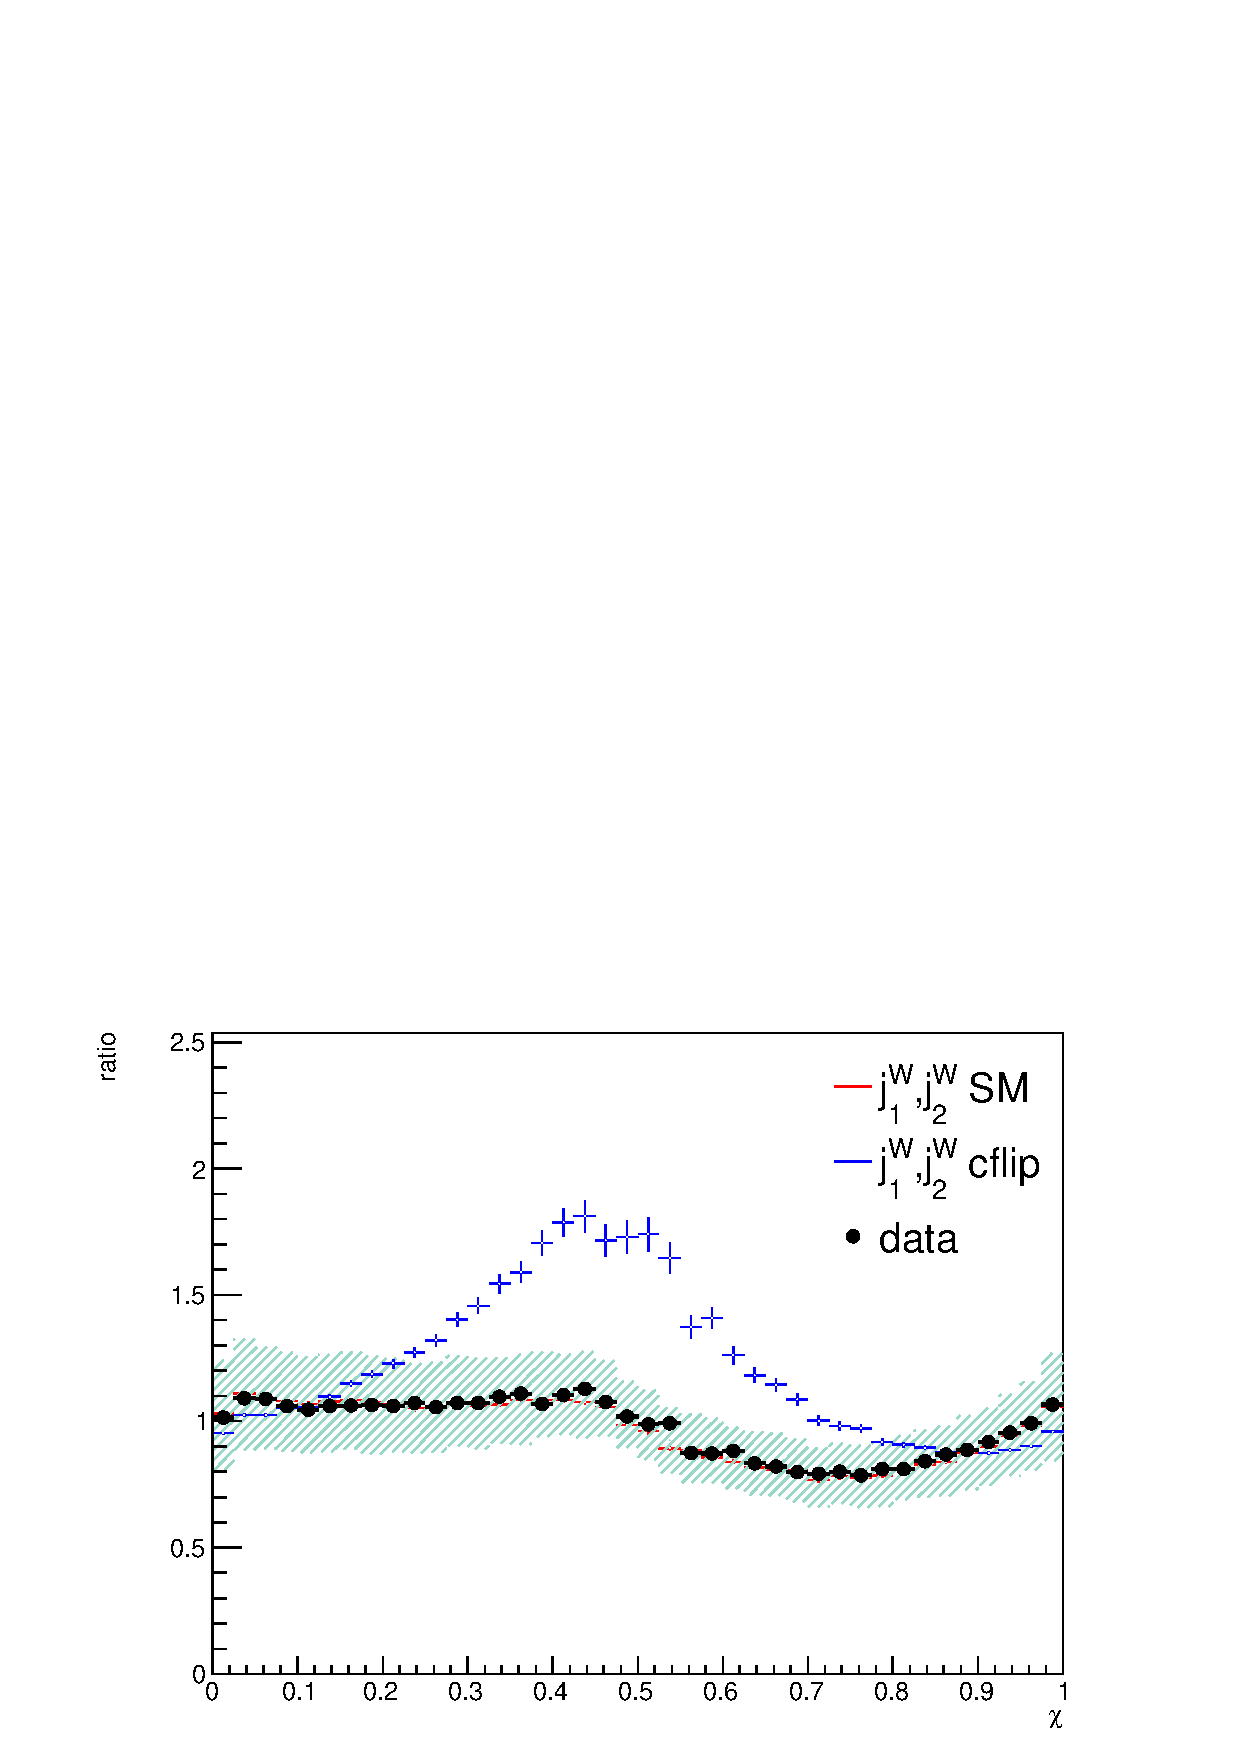
\includegraphics[width = 0.3\paperwidth]{\figrepository/ratiographs_merged_self/L_qcqf_N_allconst_reco.png}%
%%       \caption{$j_{c}^{W},j_{h}^{b}$}
%%     \end{subfigure}
%%     \begin{subfigure}[t]{0.3\paperwidth}
%%       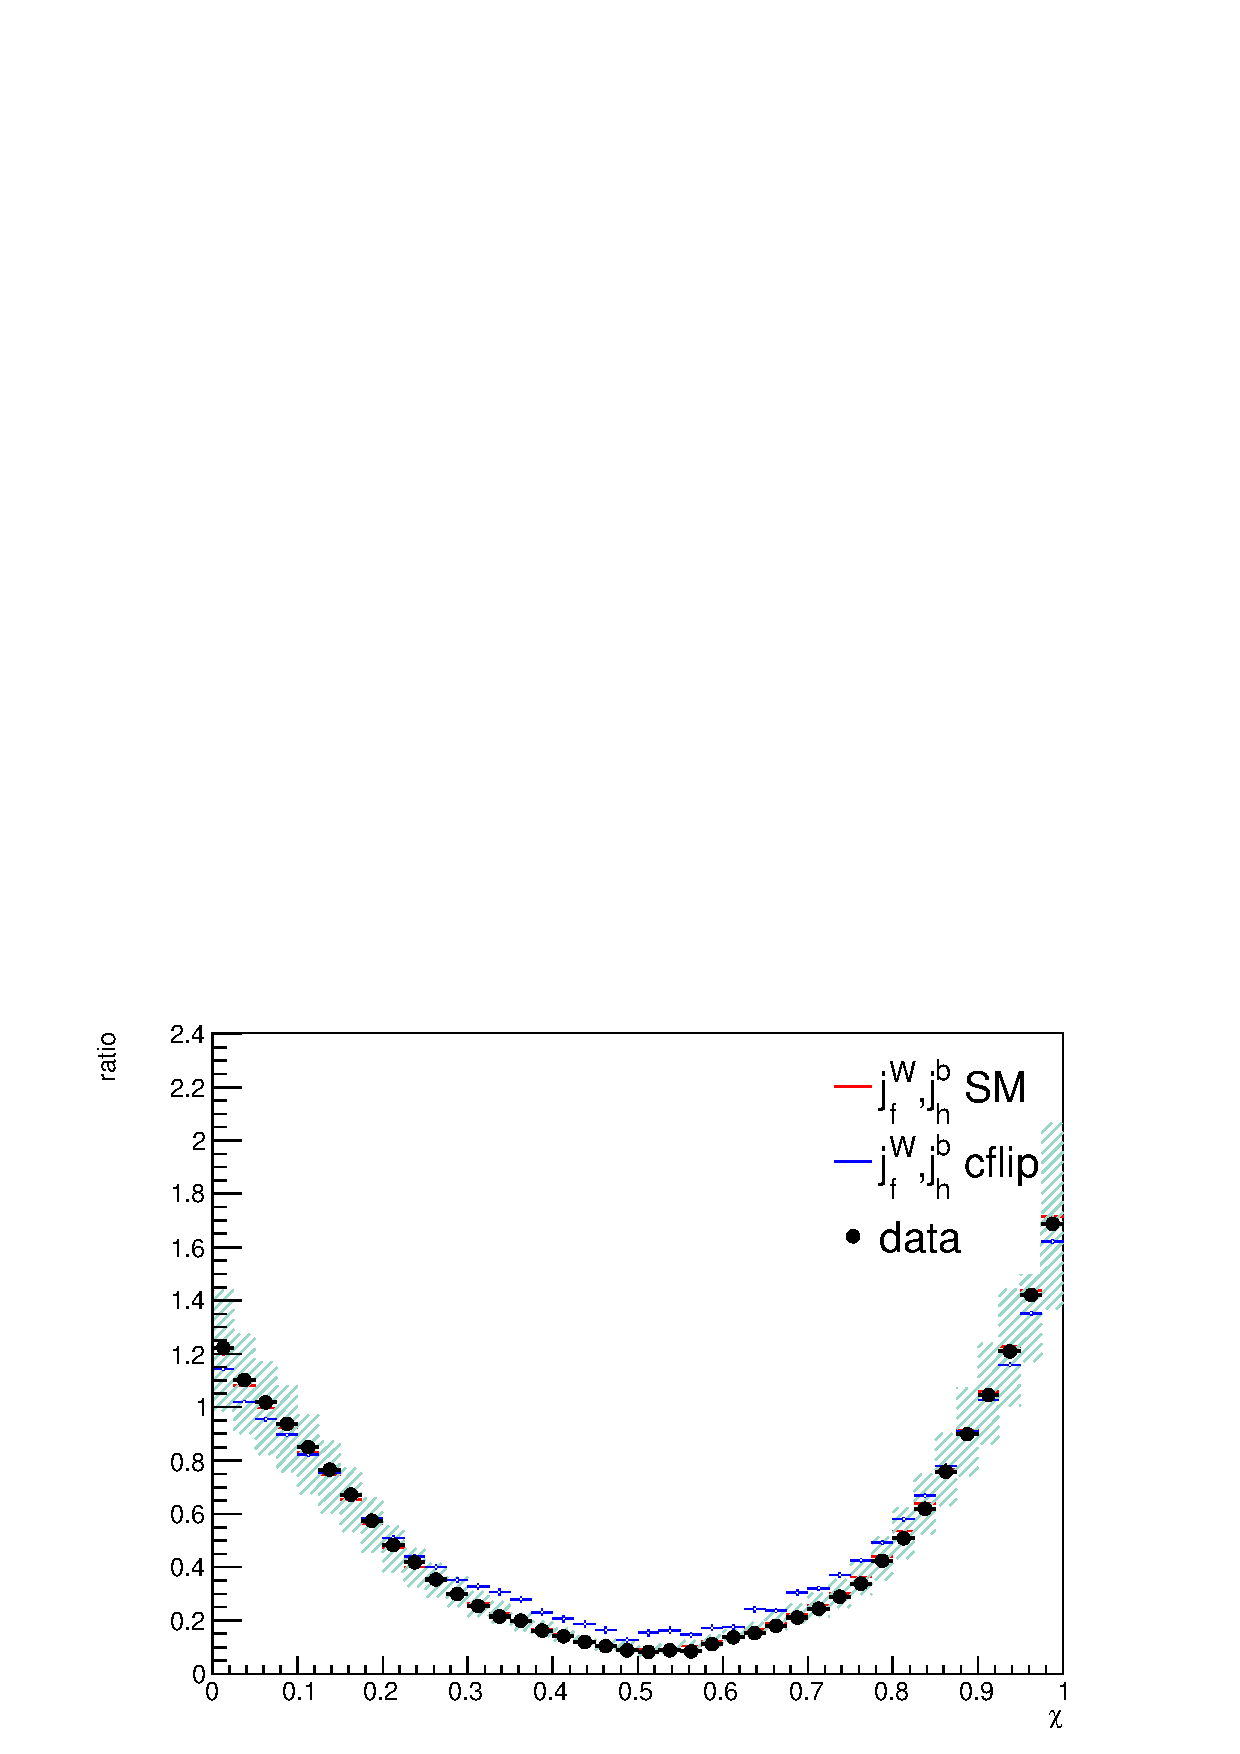
\includegraphics[width = 0.3\paperwidth]{\figrepository/ratiographs_merged_self/L_hbqf_N_allconst_reco.png}%
%%       \caption{$j_{h}^{b},j_{f}^{W}$}
%%     \end{subfigure}
%%     \begin{subfigure}[t]{0.3\paperwidth}
%%       \includegraphics[width = 0.3\paperwidth]{\figrepository/ratiographs_merged_self/L_blb2l_N_allconst_reco.png}
%%       \caption{$j_{1}^{b},j_{2}^{b}$}
%%     \end{subfigure}
%%     \caption{}
%%   \end{figure}
%% \end{frame}

%% \begin{frame}{}
  
%%   \begin{figure}
%%       \includegraphics[width = 0.8\paperwidth]{\figrepository/ratiographs_merged_SM/L_hbqc_N_allconst_reco.png}%
%%   \end{figure}
%% \end{frame}

%% \begin{frame}{}
%%   %\tiny
%%   \input{tables/Rvalues_SM/R_L_reco_MC_N_SM.txt}
%% \end{frame}

%% \begin{frame}{}
%%   %\tiny
%%   \input{tables/Rvalues_SM/R_L_reco_data_N_SM.txt}
%% \end{frame}

%% \begin{frame}{}
%%   \input{tables/Rvalues_cflip/R_L_reco_MC_N_cflip.txt}
%% \end{frame}



%% \begin{frame}{The two hypothesis model}
%%   \begin{equation}
%%     q^{TEV}=-2\ln{\frac{L(H_{0})}{L(H_{alt})}}=-2\ln{\frac{L\left(\text{data}|p=0,\hat{\theta}_{0}\right)}{L\left(\text{data}|p=P,\hat{\theta}_{P}\right)}}
%%   \end{equation}

%%   \begin{equation}
%%     n=r\left(\left(1-x\right)f_{t\overline{t}} + xf_{t\overline{t}_{\text{cflip}}}\right) + b
%%     \label{eq:n}
%%   \end{equation}
%%   \begin{figure}[htp]
%%     \includegraphics[width=\textwidth]{\figrepository/npstatistic.pdf}
%%     \caption{}
%%     \label{fig:npstatistic}
%%   \end{figure}
  
%% \end{frame}

%% \begin{frame}
%%   \begin{figure}[htp]
%%     \includegraphics[width=0.8\textwidth]{\figrepository/hypox1.png}
%%     \caption{}
%%     \label{fig:TEVx1}
%%   \end{figure}
%%   $p_{0}=0.000$\\
%%   $p_{\text{alt}}=0.000$ 

%% \end{frame}

%% \begin{frame}
%%   \begin{figure}[htp]
%%     \includegraphics[width=0.8\textwidth]{\figrepository/likelihood.png}
%%     \caption{}
%%     \label{fig:TEVx1}
%%   \end{figure}

%% \end{frame}

%% \begin{frame}
%%   \begin{figure}[htp]
%%     \includegraphics[width=0.8\textwidth]{\figrepository/hypox0335.png}
%%     \caption{}
%%     \label{fig:TEVx0335}
%%   \end{figure}
%%   $p_{0}=0.000$\\
%%   $p_{\text{alt}}=0.249$ 
%%   \end{frame}


\end{document}
